%%%%%%%%%%%%%%%%%%%%%%%%%%%%%%%%%%%%%%%%%%%%%%%%%%%%%%%%%%%%%%%%%%%%%%%%%%%%%%%%
%2345678901234567890123456789012345678901234567890123456789012345678901234567890
%        1         2         3         4         5         6         7         8
\pdfoutput=1
\documentclass[letterpaper, 10 pt, conference]{ieeeconf}  % Comment this line out
                                                          % if you need a4paper
\IEEEoverridecommandlockouts                              % This command is only
                                                          % needed if you want to
                                                          % use the \thanks command
\overrideIEEEmargins
% See the \addtolength command later in the file to balance the column lengths
% on the last page of the document



% The following packages can be found on http:\\www.ctan.org
\usepackage{graphicx} % for pdf, bitmapped graphics files
\usepackage{multicol}
\usepackage{tensor}
\usepackage{amsmath} % assumes amsmath package installed
\usepackage{amssymb}  % assumes amsmath package installe
\usepackage{array}
\usepackage{hyperref}
\usepackage{balance}
\usepackage{bm}
%\setlength{\belowcaptionskip}{-10pt}
\usepackage[detect-all]{siunitx}
\usepackage{booktabs}

\newcommand{\mv}[1]{\bm{#1}}
\newcommand{\ctrans}[3]{\tensor*[^{\mathrm{#1}}]{\mv{#2}}{_{\mathrm{#3}}}}
\newcommand{\ctransf}[4]{\tensor*[^{\mathrm{#1}}]{\mv{#2}}{_{\mathrm{#3}}^{\mathrm{(#4)}}}}
\newcommand{\sigrot}{\sigma_{\mathrm{r}}}
\newcommand{\sigtrans}{\sigma_{\mathrm{t}}}
\newcommand{\rset}{\mathcal{R}}
\newcommand{\oset}{\mathcal{O}}
\newcommand{\bset}{\mathcal{B}}
\newcommand{\uset}{\mathcal{U}}
\newcommand{\dset}{\mathcal{D}}
\newcommand{\cset}{\mathcal{C}}
\newcommand{\fset}{\mathcal{F}}
\newcommand{\eset}{\mathcal{E}}
\newcommand{\etime}[1]{\tensor*[^{\mathrm{(i)}}]{e}{_{#1}}}
\newcommand{\ejtime}[1]{\tensor*[^{\mathrm{(j)}}]{e}{_{#1}}}
\newcommand{\eztime}[1]{\tensor*[^{\mathrm{(0)}}]{e}{_{#1}}}
\newcommand{\atime}[1]{\tensor*[^{\mathrm{(i)}}]{a}{_{#1}}}
\newcommand{\ttime}[1]{\tensor*[^{\mathrm{(i)}}]{t}{_{#1}}}
\newcommand{\dt}{\Delta T}
\newcommand{\dtn}[1]{\Delta T_{#1}}
\newcommand{\dta}[1]{\tensor*[^{\mathrm{(i)}}]{\Delta a}{_{#1}}}
\newcommand{\dtaz}{\tensor*[^{\mathrm{(0)}}]{\Delta a}{}}
\DeclareMathOperator*{\argmax}{argmax}

\title{\LARGE \bf
CamSync: Synchronized Image Recording Under Large Jitter}

\begin{document}

\maketitle
\thispagestyle{empty}
\pagestyle{empty}

\begin{abstract}
Having multiple views of an object available is highly beneficial
when attempting to recover its 3D structure. If either the cameras or
the object undergo rapid motion it is necessary to synchronize the
camera shutters such that all images refer to the same point in time.
But even with hardware synchronized shutters there remains the
task of assigning the images to the corresponding synchronization
pulse as they arrive at the recording computer. This becomes
particularly difficult when high CPU load or camera link utilization
result in strongly fluctuating latencies, and simply grouping
frames by arrival time fails.
The present work describes how to utilize arrival times and embedded
image camera time stamps to reliably associate frames with sync
pulses. This scheme is implemented in CamSync, a ROS node freely available at
\href{https://github.com/daniilidis-group/cam_sync}{https://github.com/daniilidis-group/cam\_sync}.
\end{abstract}
\section{Introduction}
At first glance, recording images from hardware synchronized cameras seems a
trivial task. After all, the cameras are already synchronized, so
where is the problem?

Indeed this is straight forward when running at low frame rates over
an under utilized, reliable, low latency link such as e.g. USB3. Then
frames that are triggered by the same sync pulse will arrive as a
batch, and a simple algorithm that groups frame by time proximity will work.

Things however become tricky if for instance the receiving host has
significant CPU load that will induce occasional delays in frame arrival
times. Even more difficult are IP cameras, in particular if they are
operated at frame rates that are close to saturating the bandwidth of
the network link. Then, frames may arrive late by well more
than 1/2 of a frame period, or may be dropped at the network level
altogether. Arrival times are also affected when exposure times are
adjusted independently across cameras, compounding the problem.

Fig. \ref{fig:perioddist} shows the distribution of frame periods,
i.e. the time elapsed between consecutive frames from a single camera,
divided by the actual frame period of 25ms. While most frames are
spaced by about 25ms as expected, about 21\% arrive early or late by more than 1/2 a frame
period, and as such would be assigned incorrectly by naive time
proximity grouping.
\begin{figure}[h]
	\centering
	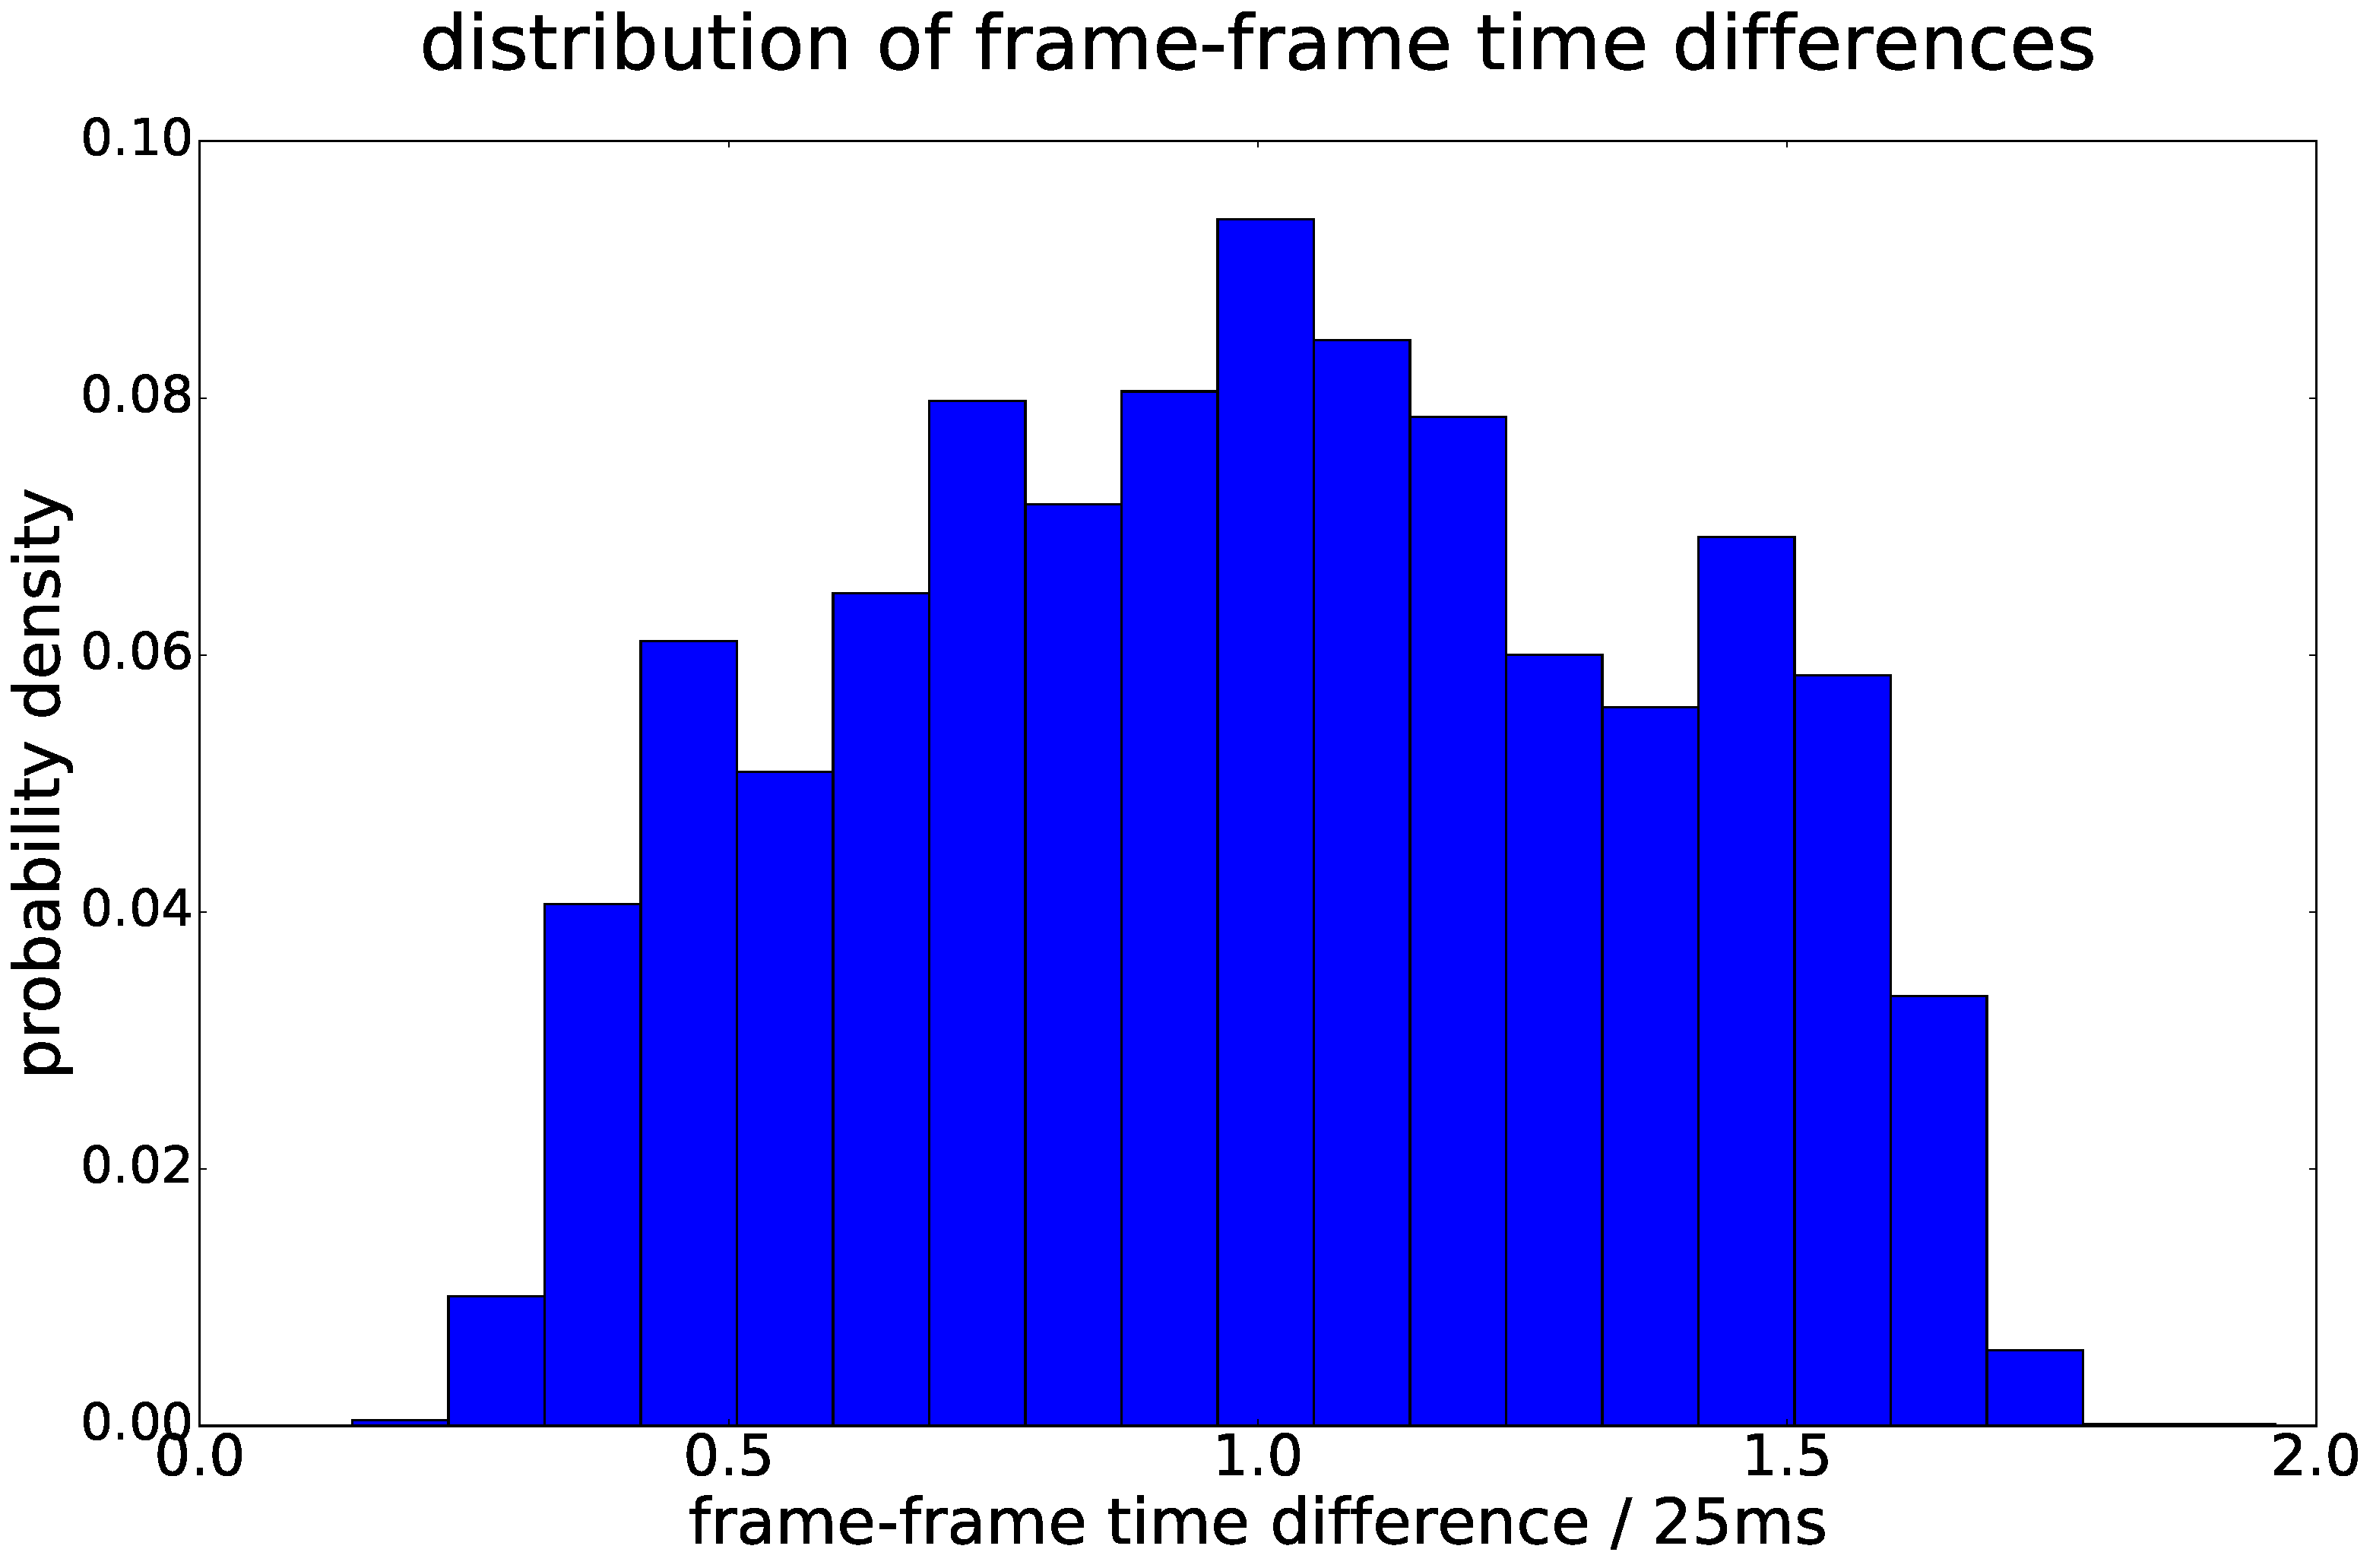
\includegraphics[width=\linewidth]{figures/period_dist.pdf}
        \caption{Distribution of frame periods, i.e. frame-to-frame time arrival
          differences for a single camera. The times have been divided
          by the sync pulse period of 25ms, such that a value of 1
          along the x axis corresponds to two frames that have arrived
          exactly  25ms apart.}
    \label{fig:perioddist}
\end{figure}

Fig. \ref{fig:arrival_vs_frame} illustrates this more clearly. Along
the $x$ axis it shows the ``true'' frame time $T$ (more about this in
section \ref{sec:sync_algo}), along the $y$ axis the actual time the
corresponding images arrived at the host. One can see that by the time
the last image corresponding to one sync pulse arrives, the first one
for the next sync pulse follows right
away. In Fig. \ref{fig:arrival_vs_frame}, all arrival time stamps have
been aggregated into a vertical line at time stamp 137.85s to
demonstrate how difficult it is to recover frame boundaries just by
looking at arrival time stamps.
\begin{figure}[h]
	\centering
	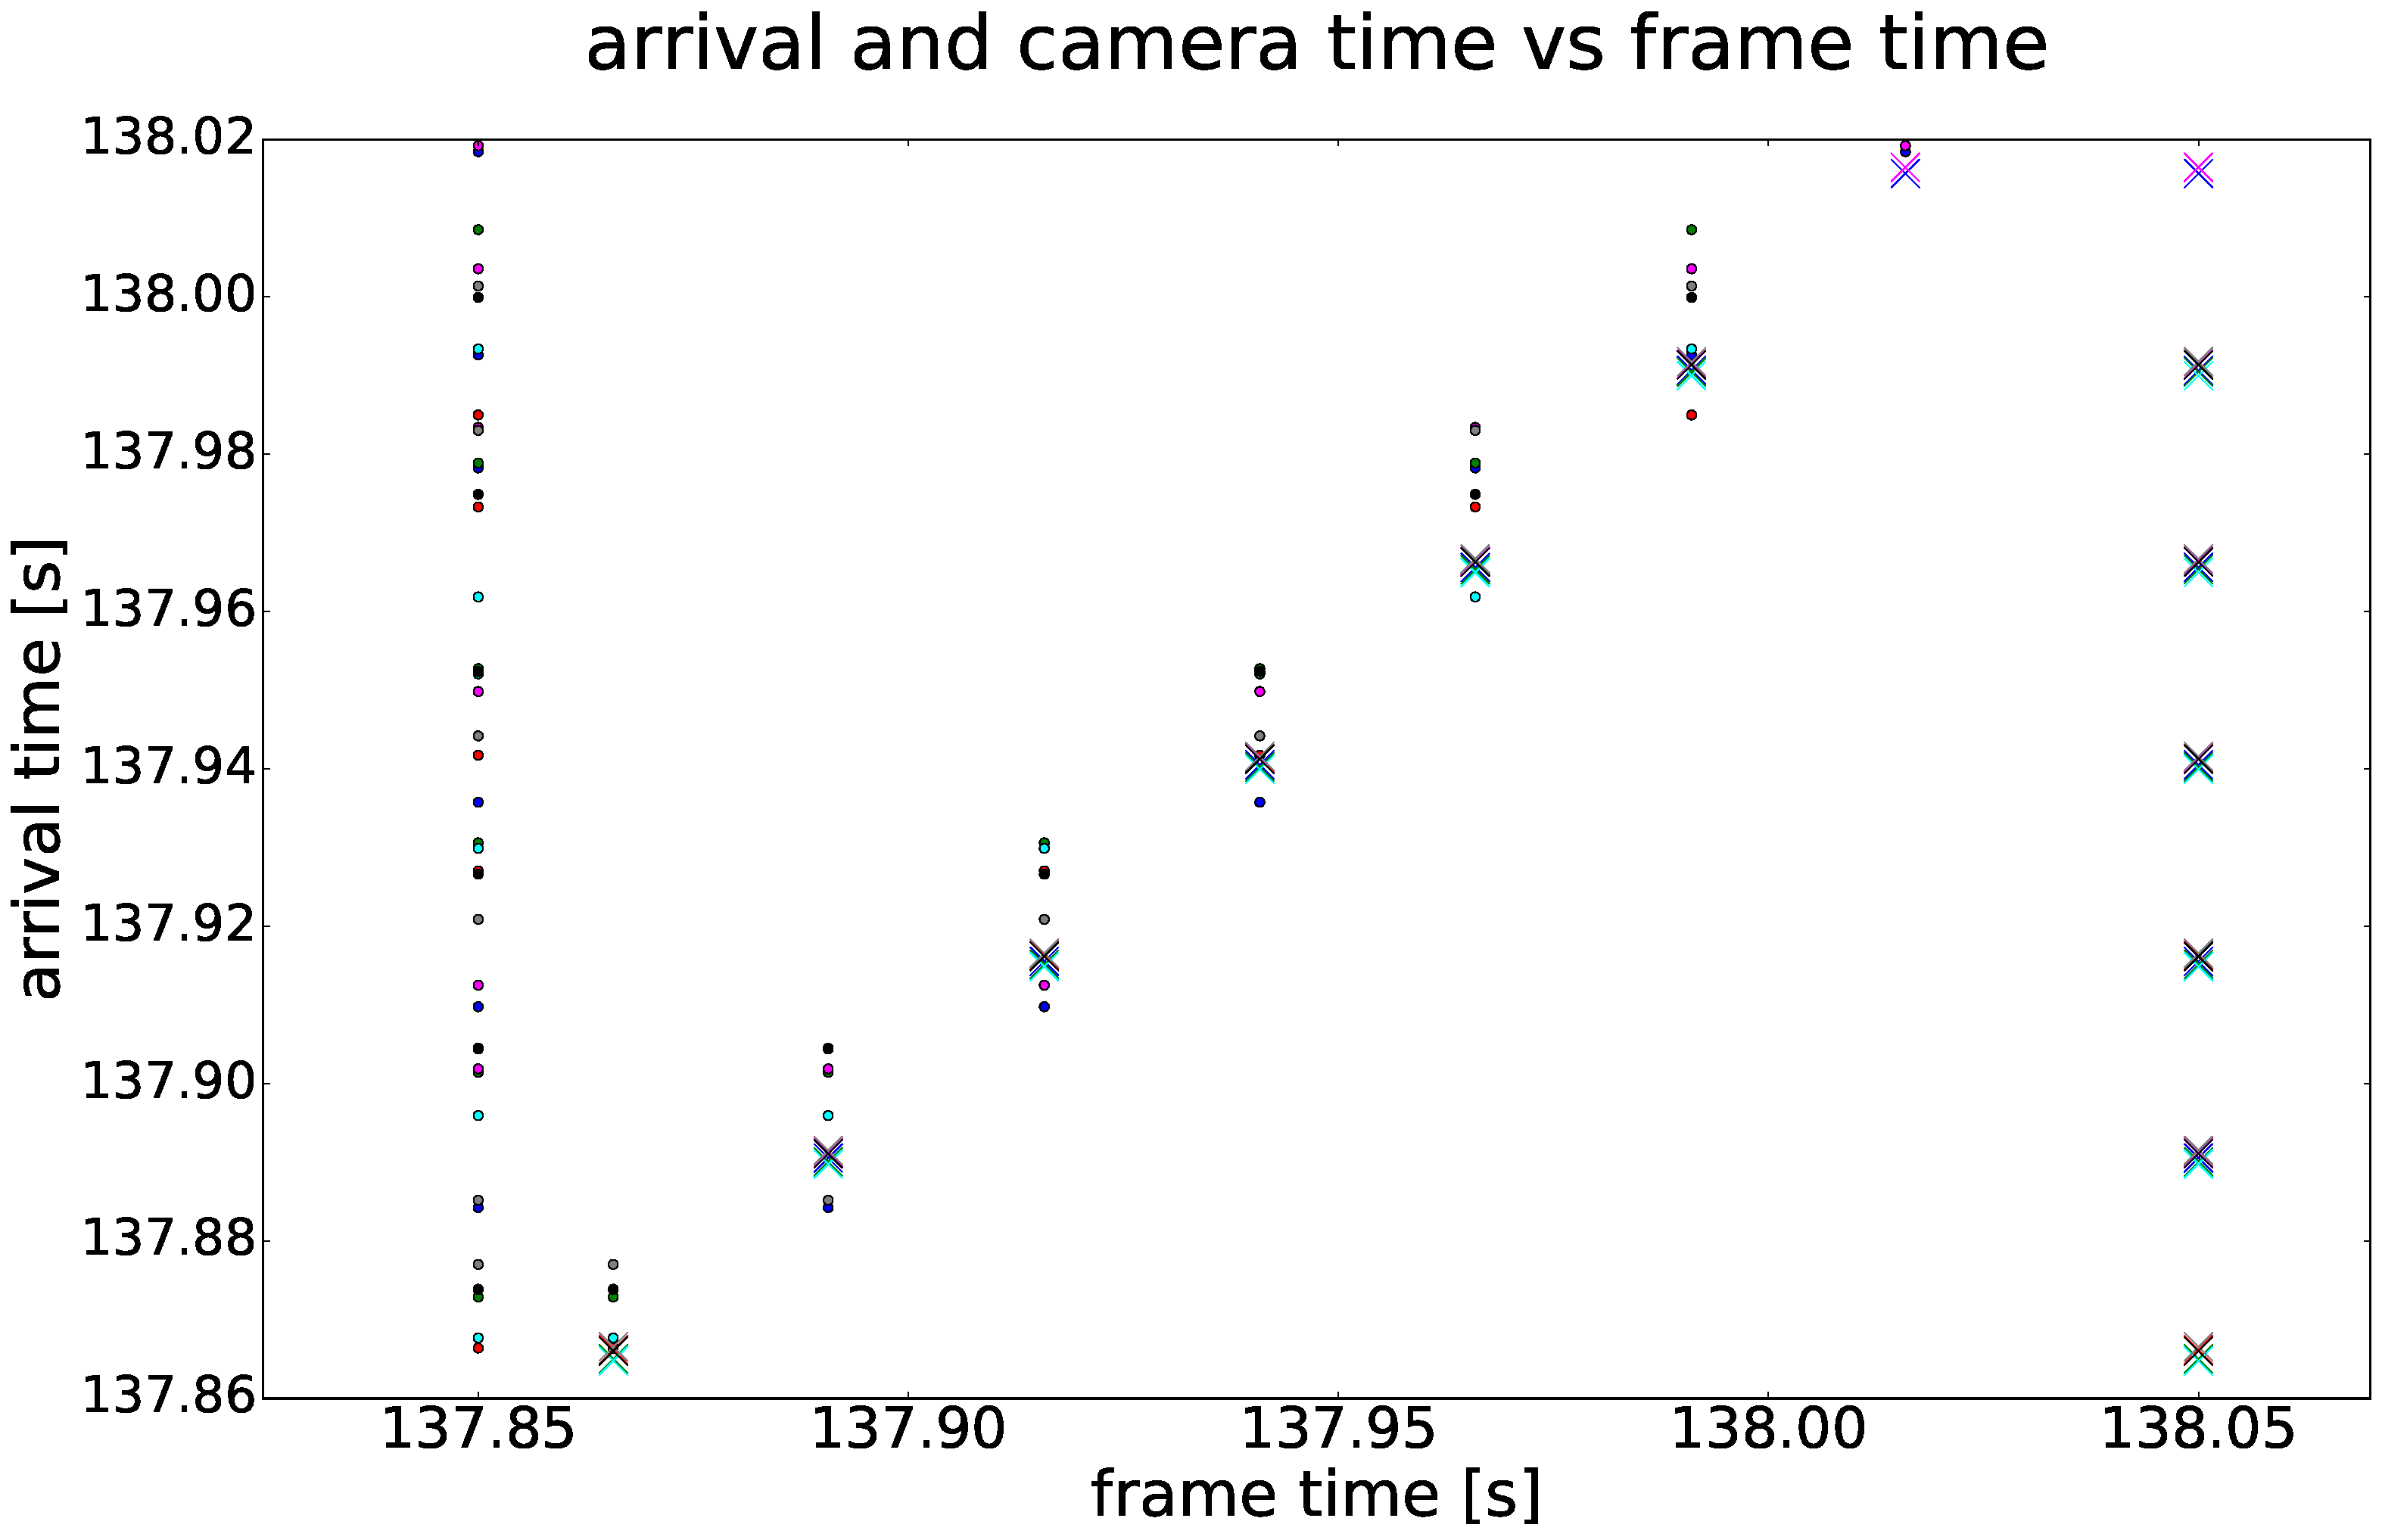
\includegraphics[width=\linewidth]{figures/arrival_vs_frame.pdf}
        \caption{
          Time of arrival $\atime{}$, filled circles, and
          camera time, $\ttime{}$, crosses, plotted vs the sync pulse
          time $T$. The color indicates the camera index $i$. To
          visualize how challenging it is to group frames based on
          arrival time only, all arrival times have been collapsed onto a
          single frame at $T$=137.85s. Grouping by the filtered camera
          time $\ttime{}$ however is straight forward, as is shown at $T$=138.05s.}
    \label{fig:arrival_vs_frame}
\end{figure}

Fortunately many computer vision cameras offer the option to embed 
camera time stamps right at the imager, before the frame is sent over
the wire. Although the clocks on the cameras are offset with
respect to each other, and will drift over time, they provide a way to
reliably detect dropped frames, which is crucial for removing jitter
from the arrival times.

After several failed attempts, we eventually found a robust method
of assigning time stamps to frames. Moreover, our method has good diagnostic
capabilities and reliably produces alerts when synchronization is no
longer possible due to e.g. failed 
hardware synchronization or excessive CPU load.

This paper documents the lessons learned during the
implementation. The method described here is implemented in the ROS
\cite{ros} ``CamSync'' node, which we hope will be useful for other projects
that require accurate synchronized timestamps in a multi-camera
setting. The code can be found at
\href{https://github.com/daniilidis-group/cam_sync}{https://github.com/daniilidis-group/cam\_sync}.

\section{Hardware Setup}
\begin{figure}[h]
	\centering
	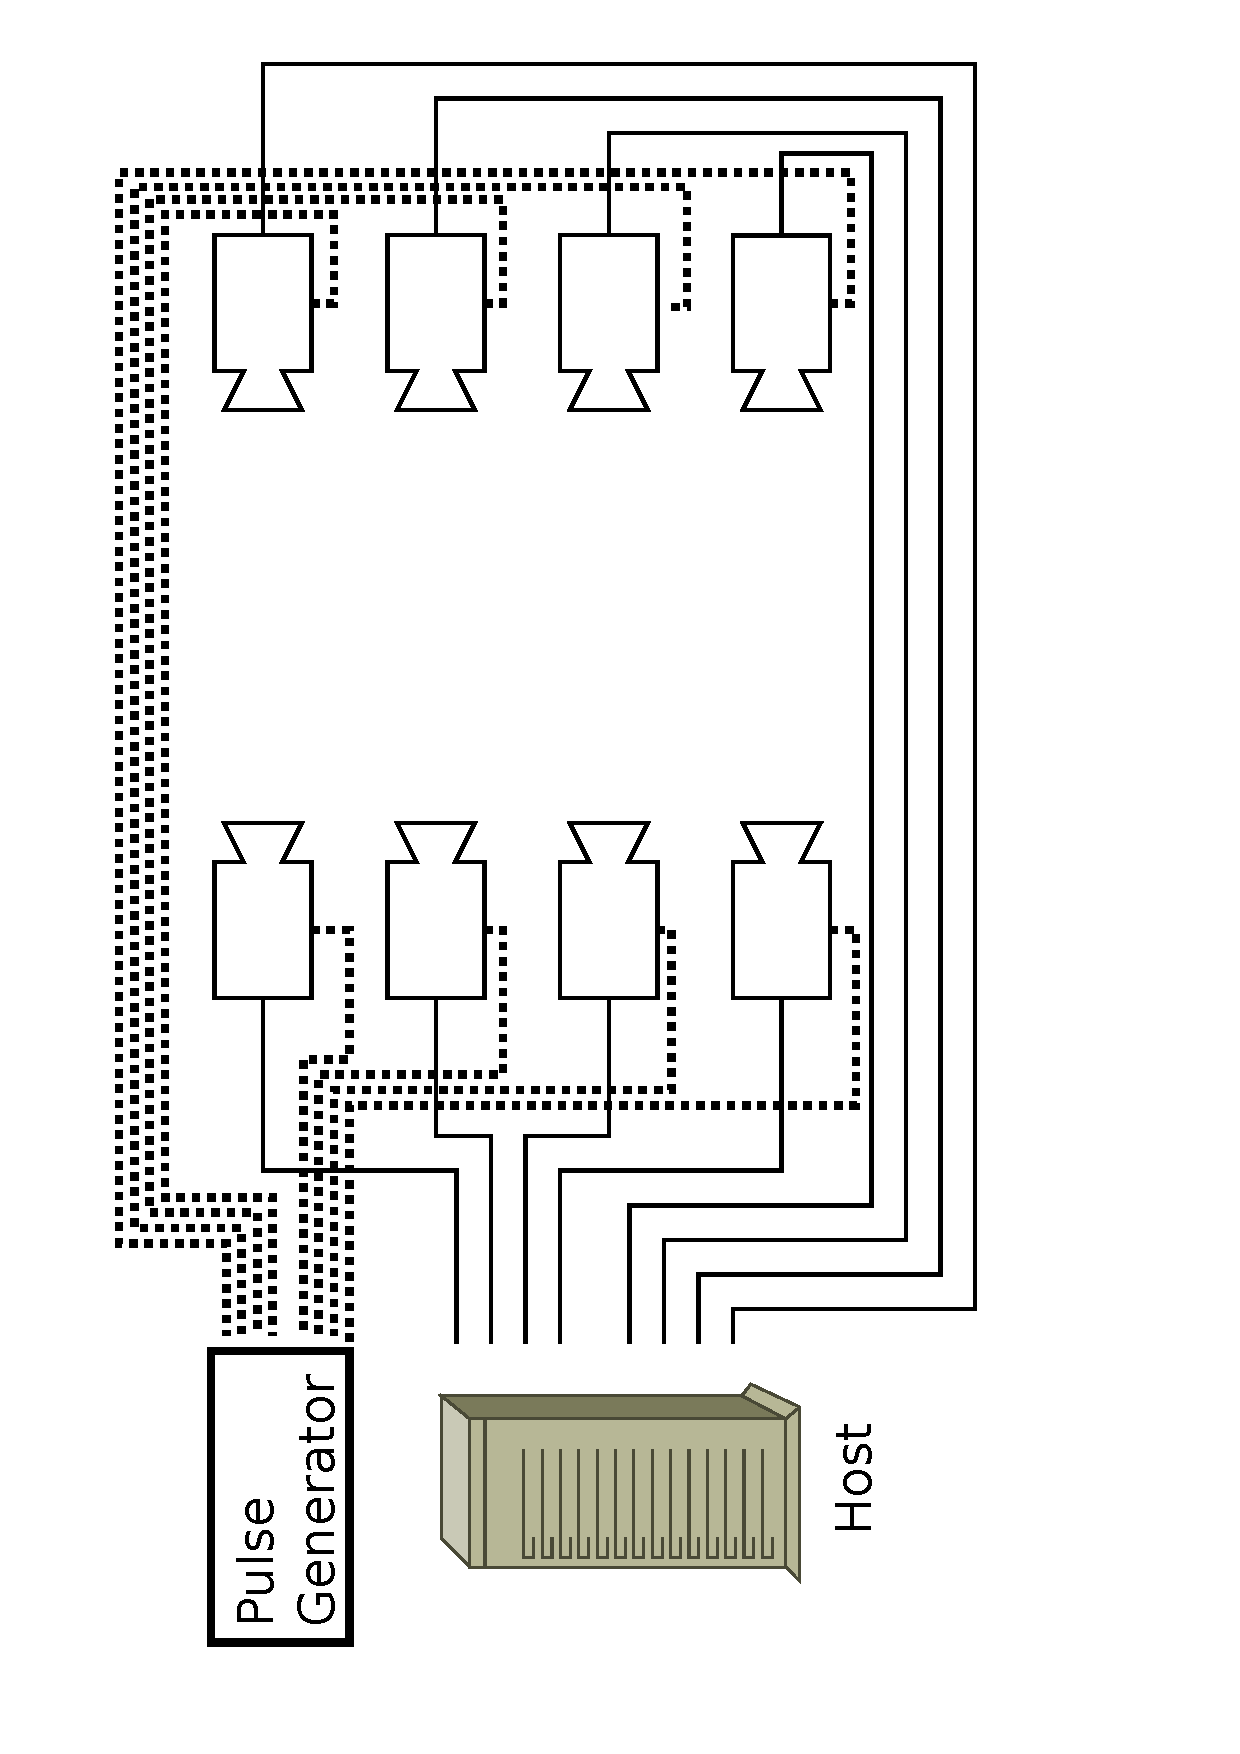
\includegraphics[angle=-90,width=\linewidth]{figures/ip_cameras.pdf}
        \caption{Eight FLIR/PointGrey IP cameras are directly
          connected via Gigabit Ethernet (GigE) directly to two 4-port
          network cards at the host. An external pulse generator
          (PixHawk) is used to trigger the cameras.}
    \label{fig:gige_setup}
\end{figure}
In this section we briefly go over the hardware setup, shown in
Fig. \ref{fig:gige_setup},  with which the experimental data was collected.

Eight Gigabit Ethernet color cameras (FLIR BFLY-PGE-23S6C-C) are located
up to about 7m apart and are facing each other. The cameras utilize a 1" Sony
Pregius IMX249 global shutter sensor which offers an image resolution of
1920x1200 at up to 41 Hz. Shielded CAT6E twisted pair copper cables
transport the data over a 
distance of about 15m to a central host. The camera shutters are
triggered synchronously at 40Hz (1ms strobe duration) by an external pulse generator, in
this case a PixHawk running the PX4 flight stack, which has a feature
to generate an external TTL pulse at 3.3V.

\begin{figure}[h]
	\centering
	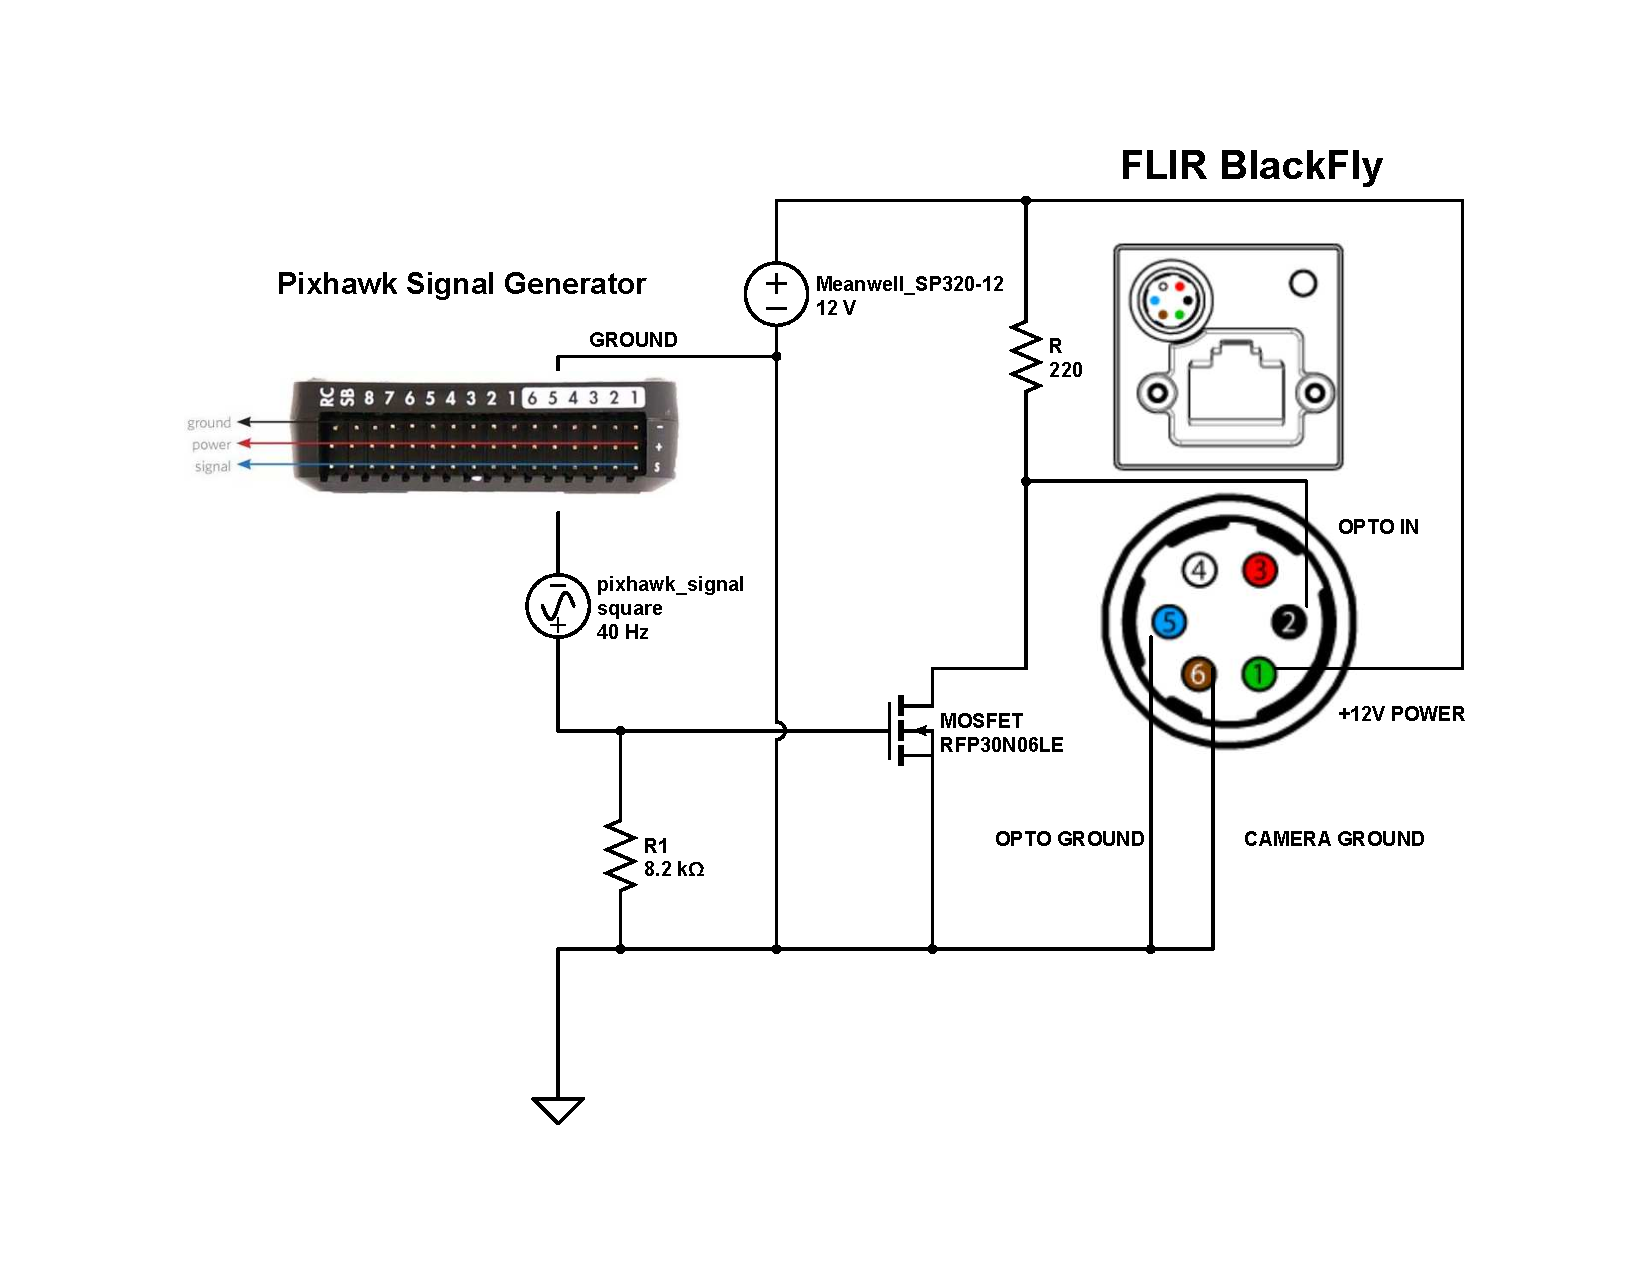
\includegraphics[width=\linewidth]{figures/aviary_sync_circuit.pdf}
        \caption{Circuit for driving the GPIO sync pin of eight FLIR/PointGrey Blackfly
          cameras from a PixHawk 3.3V TTL pulse. The signal is too
          weak to drive the eight opto-coupled input ports of the
          cameras, and is therefore amplified by a TTL MOSFET.}
    \label{fig:sync_circuit}
\end{figure}

Unfortunately, the signal from the PixHawk is not strong enough to
drive all eight camera input pins. The required amplifier circuit is
shown in Figure \ref{fig:sync_circuit}. In this configuration, the
signal to the cameras has a peak of 6V, which is well above the 3V
required to drive the opto coupler. If more 
cameras are connected and the signal gets too weak, a 
smaller resistor R should be used.

When running at 40Hz, transmitting a camera's raw Bayer
images will already consume 737Mbits, not including network packet
overhead. This is just within the capacity of a 1Gbit link, and will
put signficant load on camera, network card, and host driver.

\section{Synchronization Algorithm}
\label{sec:sync_algo}
\subsection{Outline}
The ultimate objective of synchronized recording is to assign
the identical timestamp $T_n$ to all camera frames that are triggered
by the $n$-th synchronization pulse. This global time $T_n$ should
advance at a near constant rate with low jitter, and should on average correspond to the
time at which the frames arrive at the host.

When sync pulse number $n$ triggers a frame, two different sources of
timing information become available:
\begin{enumerate}
\item
The image time stamp $\etime{n}$ embedded with the image from camera
$i$. While the corresponding set of time stamps $\etime{}$ has low jitter,
it is generated by the camera, and can 
therefore not be directly compared to the host clock. Moreover, $\etime{}$
may drift over time from $\ejtime{}$, since the camera clocks are not disciplined. For
this reason we use the embedded timestamps only
for detecting dropped frames. For that purpose however, they are
indispensible.
\item
The time $\atime{n}$ when the frame from camera $i$ arrives at the
application layer. Although the set of arrival times $\atime{}$ is plagued
by large noise (cf Fig. \ref{fig:perioddist}), $\atime{}$ is consistently
measured by the host clock across all cameras. To be precise,
$\atime{n}$ is the time of arrival of frame $n$ from camera $i$,
{\em minus the current shutter time of camera $i$}. Subtracting off the
shutter time removes the systematic bias due to the fact that cameras
with longer shutter time settings will send their images later. So
although we will subsequently refer to $\atime{}$ as the arrival time,
it really is the arrival time {\em net of shutter time}.
\end{enumerate}

With these preliminary definitions, we can outline our strategy, which
consists of three steps:
\begin{itemize}
\item First, we establishes a low jitter estimate of the strobe period
  $\dt$. The strobe period is an estimate of the true time (as measured
  measured by the host clock) that elapses between sync pulses
  triggering the cameras.
\item With known strobe period, we maintain a per-camera clock
  $\ttime{}$ that upon
  frame arrival is advanced by the strobe period. The per-camera clock
  will thus inherit the low jitter property from the strobe
  period. While the arrival times $\atime{}$ may temporarily deviate
  from the corresponding times $\ttime{}$, on the long run and on average, $\ttime{}$ and
  $\atime{}$ agree. This is mainly due to the fact that $\ttime{}$ is updated with the ``true''
  strobe period $\dt$. An additional small correction term is added to
  the camera clock update to remove possible   drift.
\item Once a low-jitter per-camera clock is available, simple time
  proximity can be used to determine if a newly arriving frame
  can be associated with ones that have already been received, or
  if it is the first frame corresponding to the next sync pulse.
\end{itemize}

Fig. \ref{fig:arrival_vs_frame} shows the dramatic reduction of jitter
when going from raw arrival times $\atime{}$, shown as filled circles,
to the filtered camera times $\ttime{}$,
shown as crosses. The following subsections will describe in detail
how the filtering works.

\subsection{Estimating the strobe period}
Based on the frequency $f$ to which the pulse
generator is set, an initial estimate of the strobe period can be computed as
$\dt_0 = 1/f$. This serves as a starting point for an 
exponential moving average, which is updated whenever a new camera strobe period $\dta{n}$
becomes available for any camera $i$:
\begin{equation}
\label{eq:expavg}
\dtn{n} = (1-\alpha) \dtn{n-1}  + \alpha\ \dta{n}\ .
\end{equation}
Because of the possiblity of frame drops, the camera strobe period
$\dta{n}$ cannot simply be determined by subtracting $\atime{n-1}$
from $\atime{n}$. Rather, we first use the embedded image timestamps $\etime{}$
to find the number of frames that have passed:
\begin{equation}
\label{eq:nframes}
 k = \mathrm{round}((\etime{n} - \etime{\mathrm{prev}})/\dtn{n})\ .
\end{equation}

Then the strobe period for a camera is simply the time difference
of arrival times between two frames, divided by the number of frames:
\begin{equation*}
\dta{n} =  \frac{\atime{n} - \atime{n-k}}{k}\ .
\end{equation*}

The coefficient $\alpha$ in Eq. \ref{eq:expavg} is set such
as to average over a time horizon that is longer than any temporary
latency fluctuations, for instance $\tau=10$ seconds:
\begin{equation}
\alpha = 1/(f N \tau)\ .
\end{equation}

Fig. \ref{fig:expavg} shows the estimated $\dt$ as a function of
time. Notice how during the first few seconds the estimate is not well
established. During this warmup period, no frames are published.

\begin{figure}[h]
	\centering
	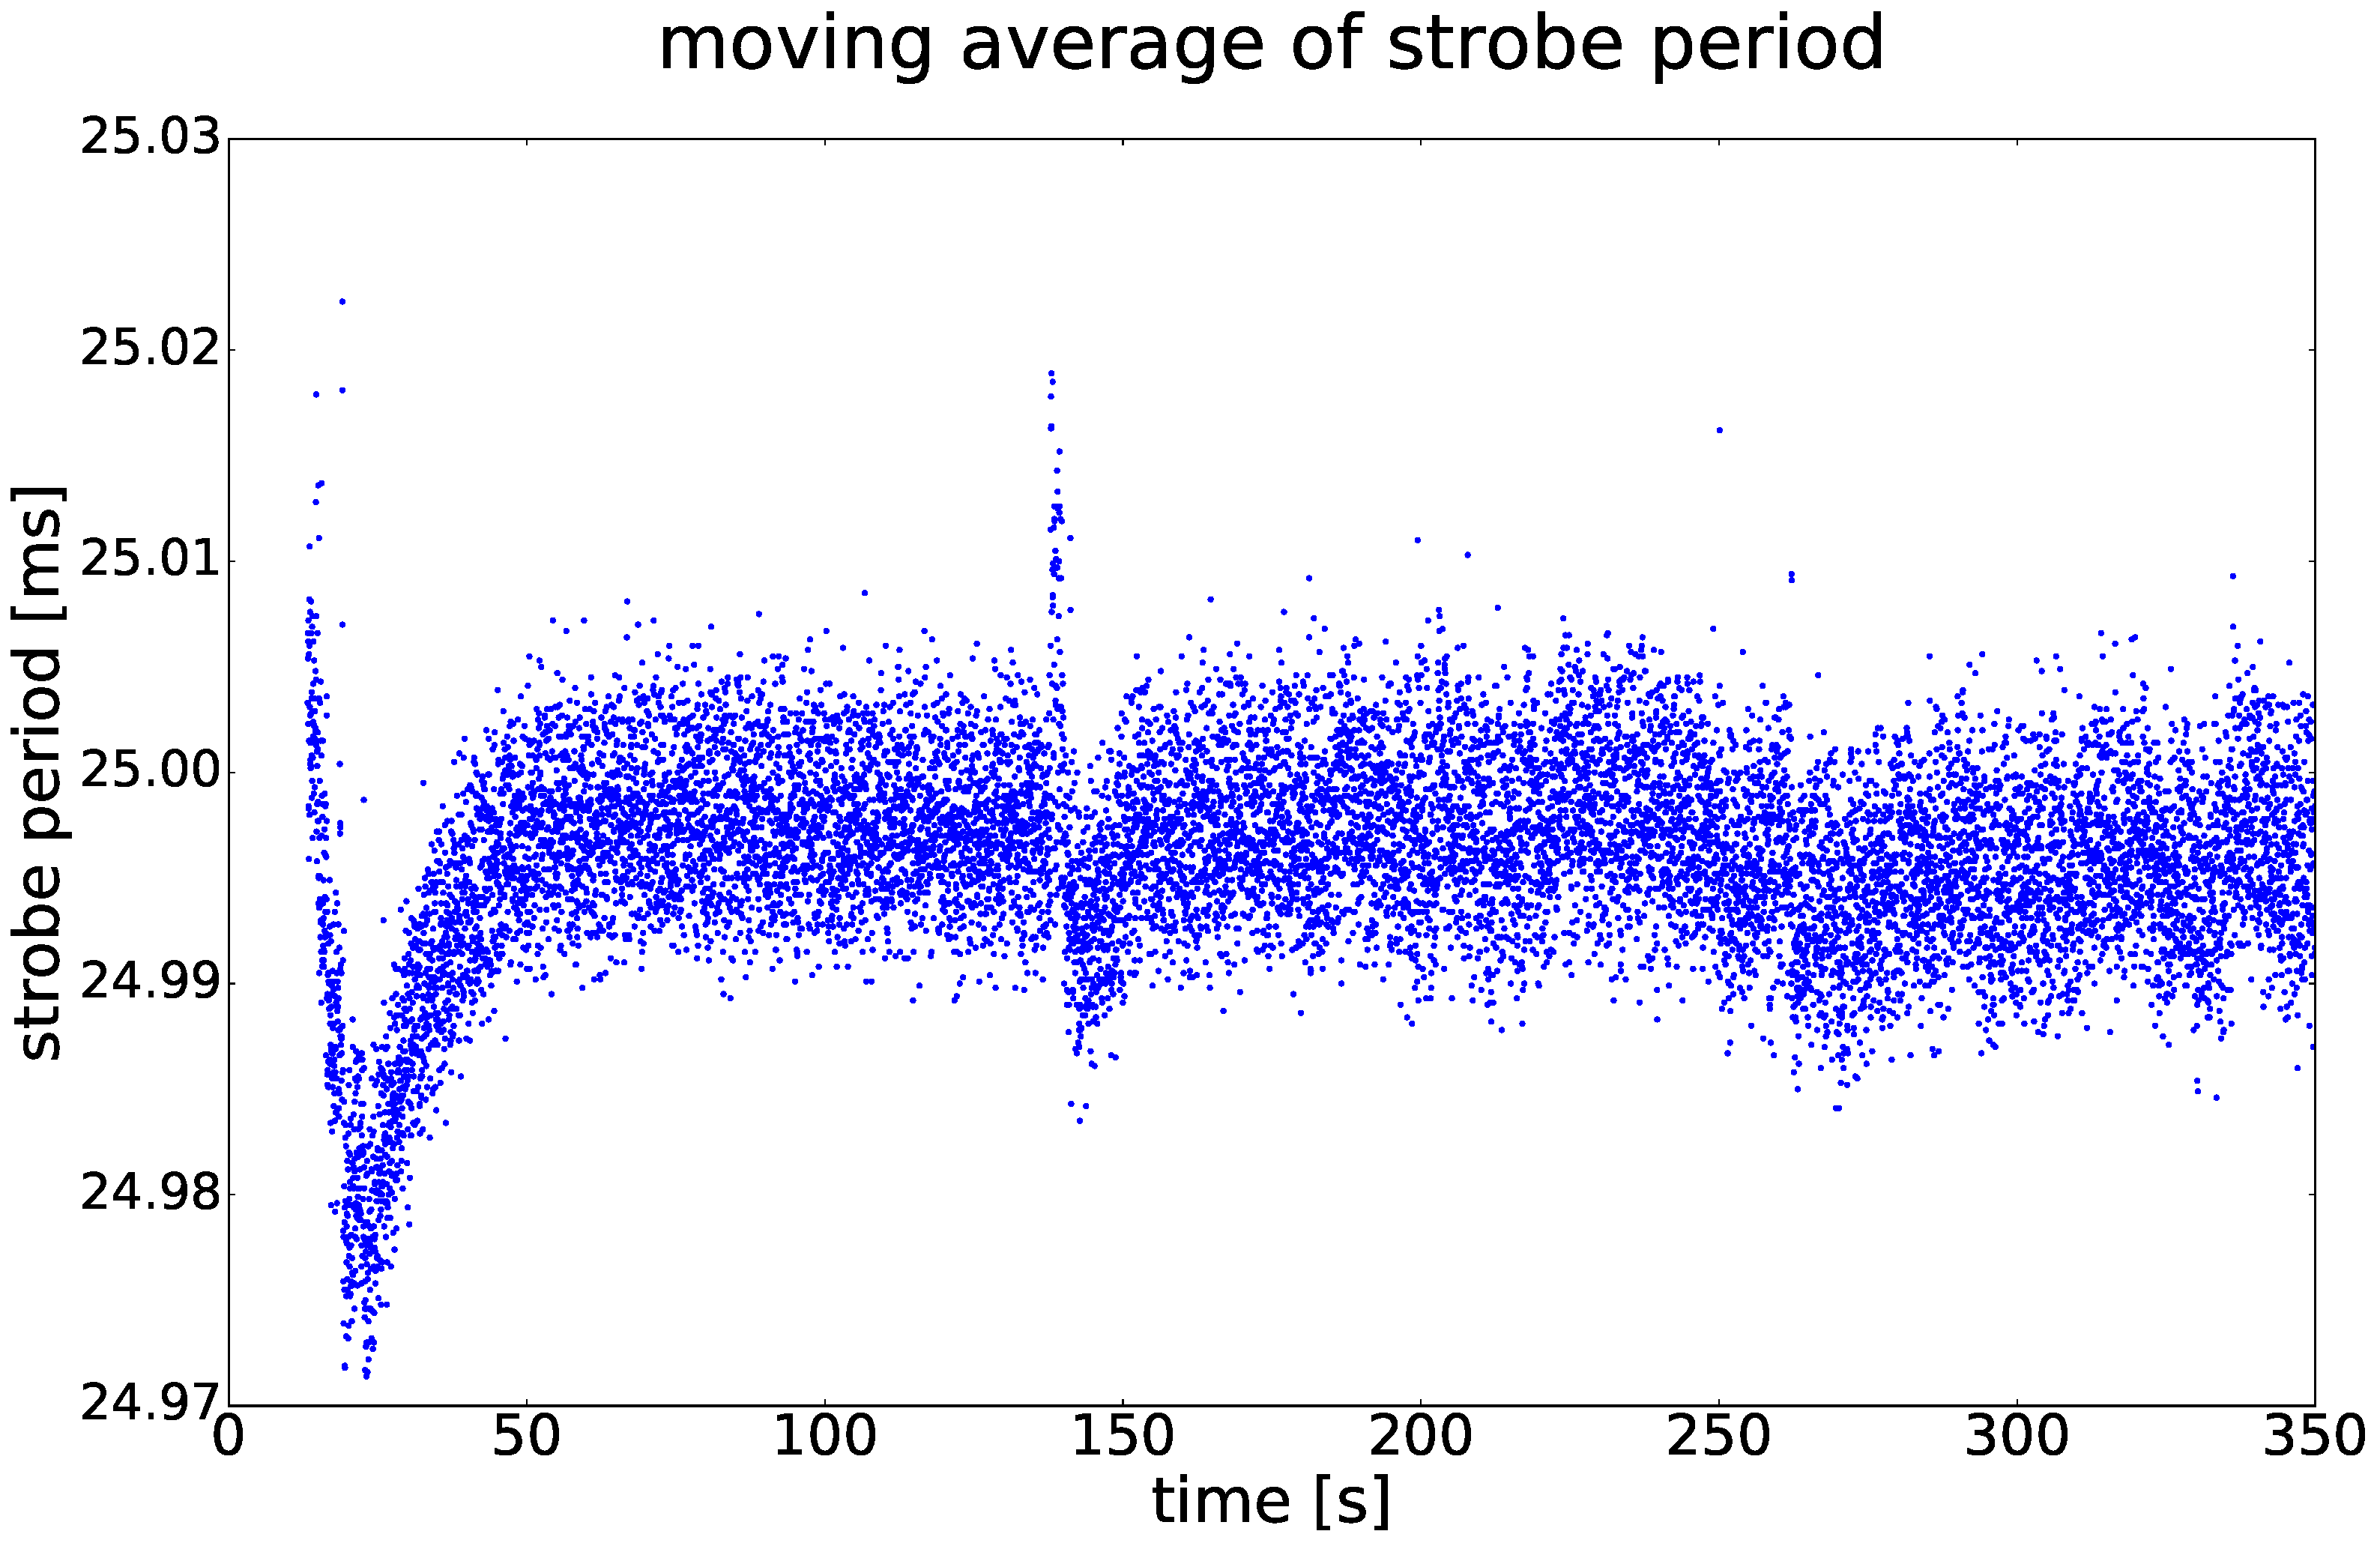
\includegraphics[width=\linewidth]{figures/exp_avg_warmup.pdf}
        \caption{After a short warmup time, the estimated strobe period $\dt$ converges to
          a value of 25ms corresponding to $f=40$Hz. The peak at 140s is
          due to a spike in CPU load caused by a client ROS node
          subscribing to camera images.}
    \label{fig:expavg}
\end{figure}

Due to the scale of the $y$ axis, the strobe period $\dt$ in Fig. \ref{fig:expavg}
seems noisy. However, this must be put into
perspective. Fig. \ref{fig:raw_dt} shows the strobe period $\dtaz$ computed
from raw differences in 
arrival times for camera 0. Compared to the large
noise of the input data, the average (shown in blue) is actually very stable.

\begin{figure}[h]
	\centering
	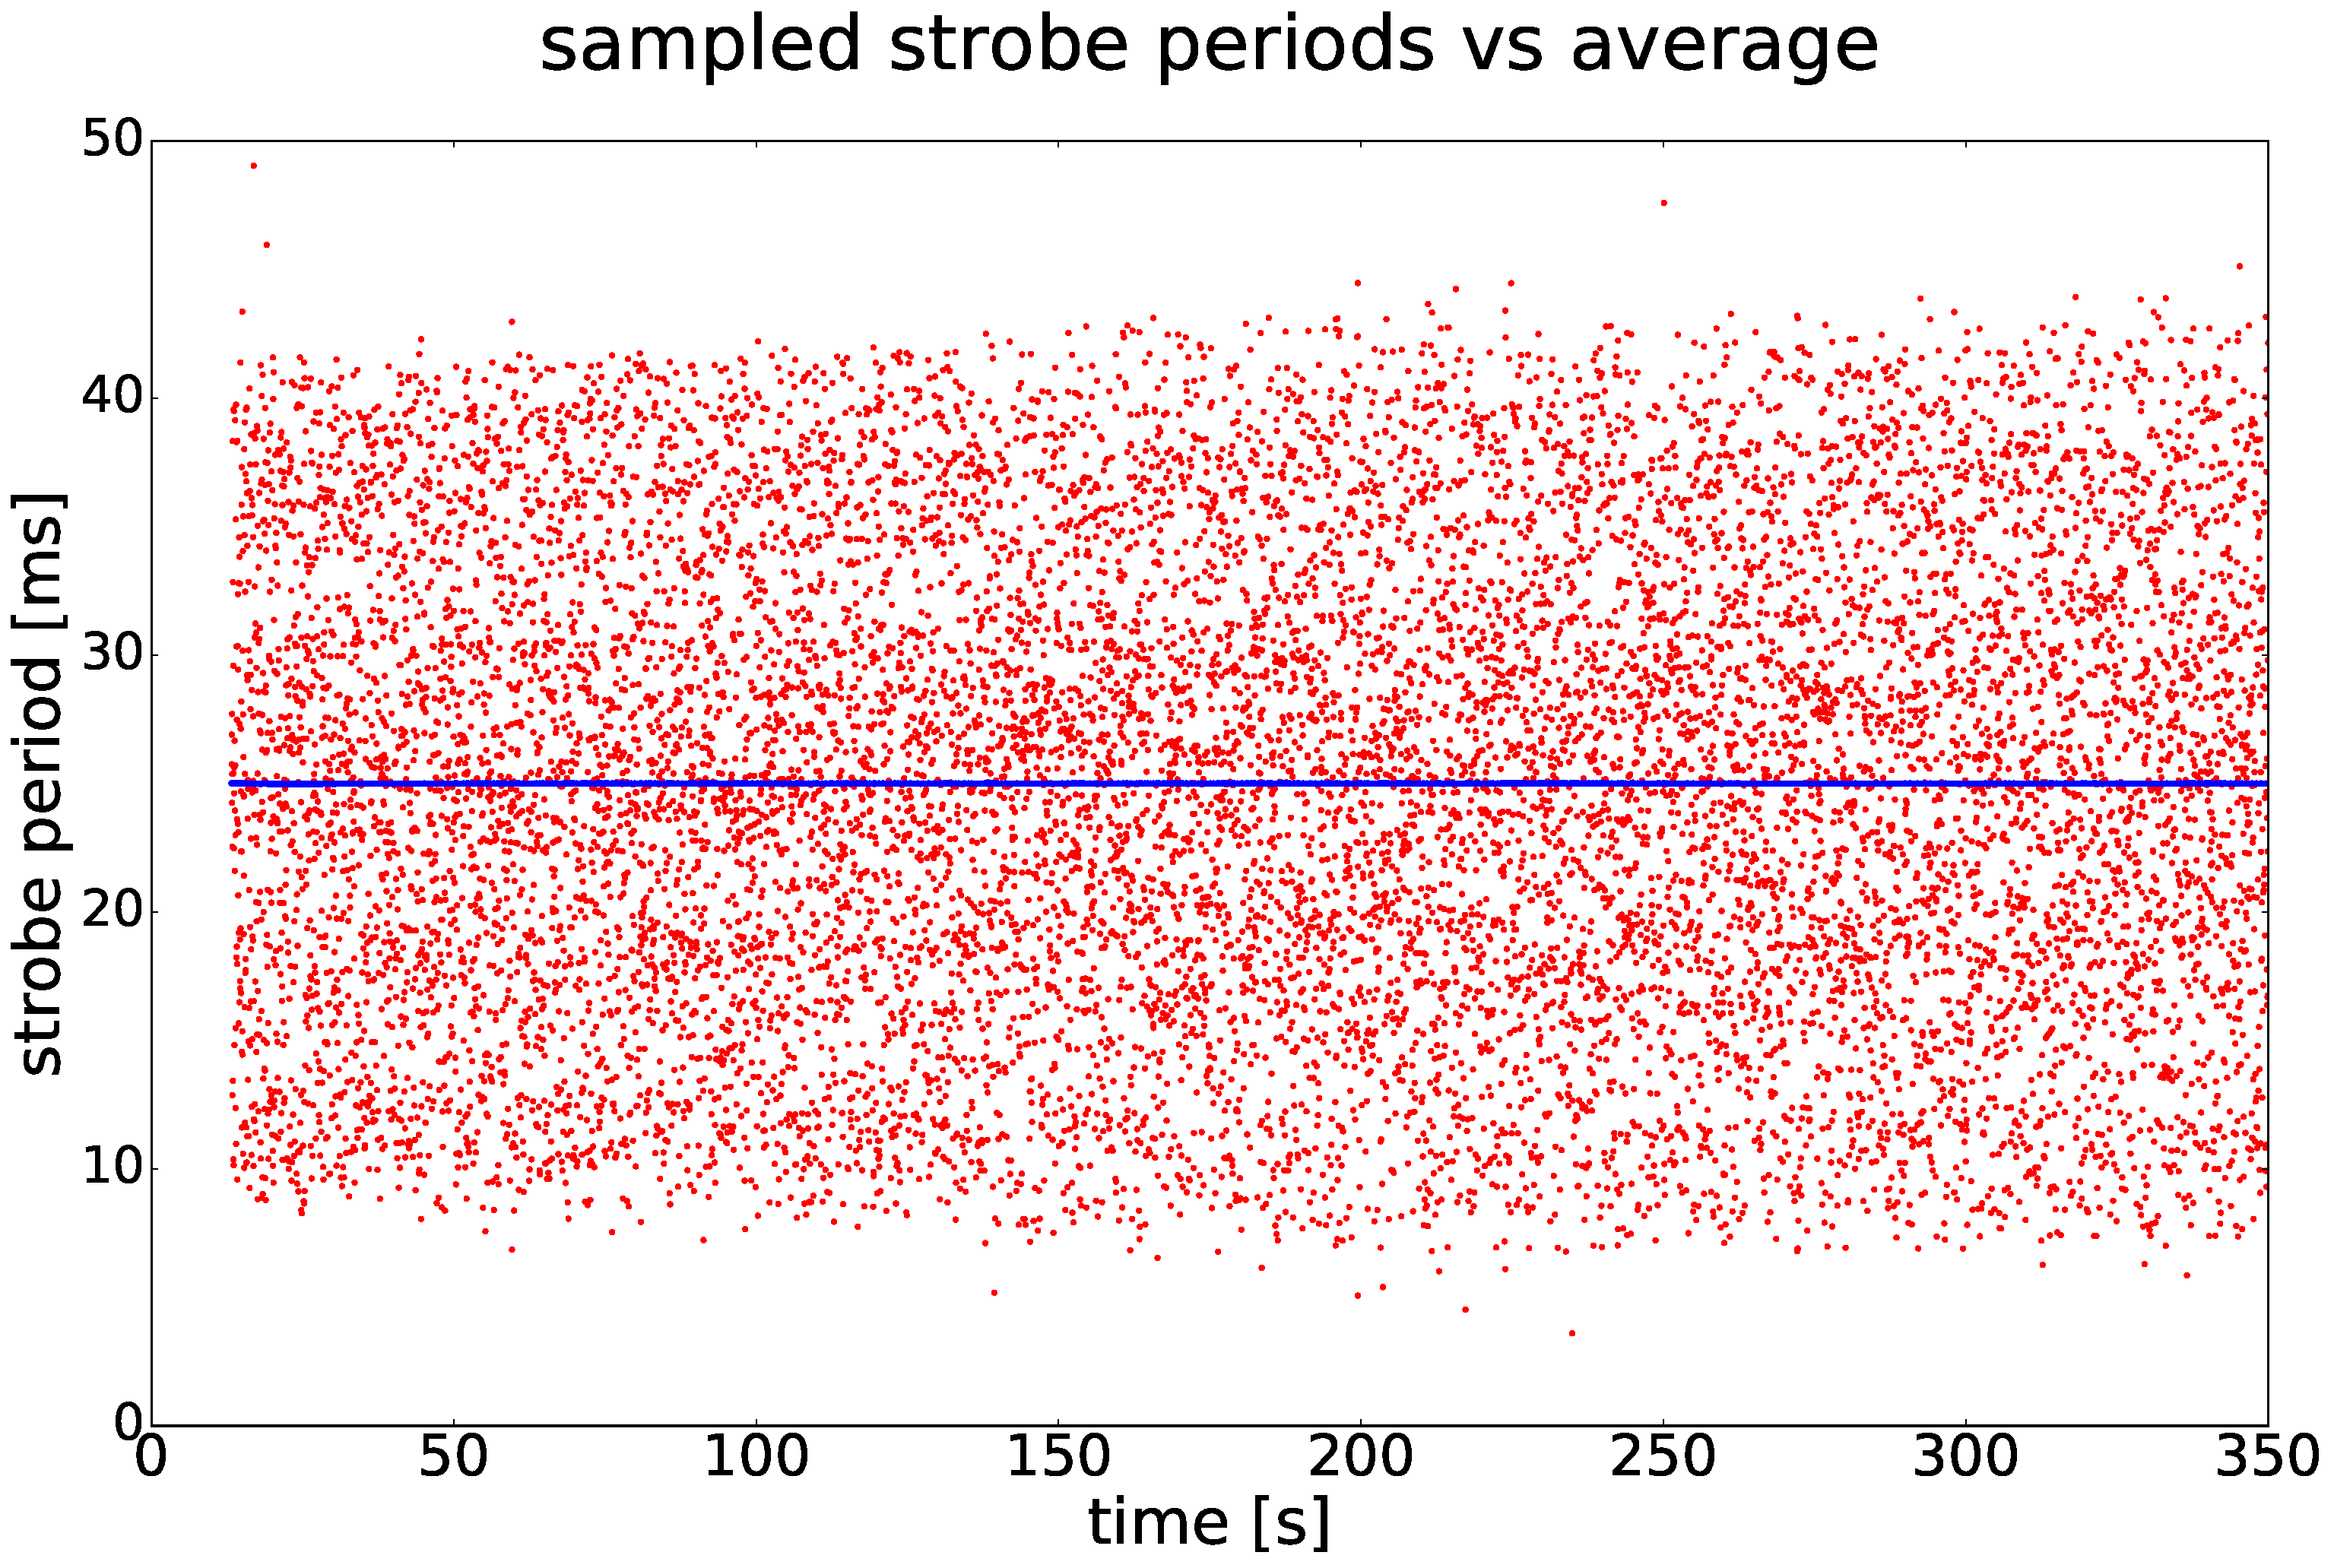
\includegraphics[width=\linewidth]{figures/samples_vs_avg.pdf}
        \caption{Red dots: strobe periods $\dtaz$,
          from camera 0 arrival time differences. Blue dots:
          $\dt$, computed by 10s exponential moving average
          over all camera strobe periods.}
    \label{fig:raw_dt}
\end{figure}

It turns out that $\dt$ is also more stable than differences of
embedded image time stamps. Fig. \ref{fig:embed_dt} shows this cleary.
\begin{figure}[h]
	\centering
	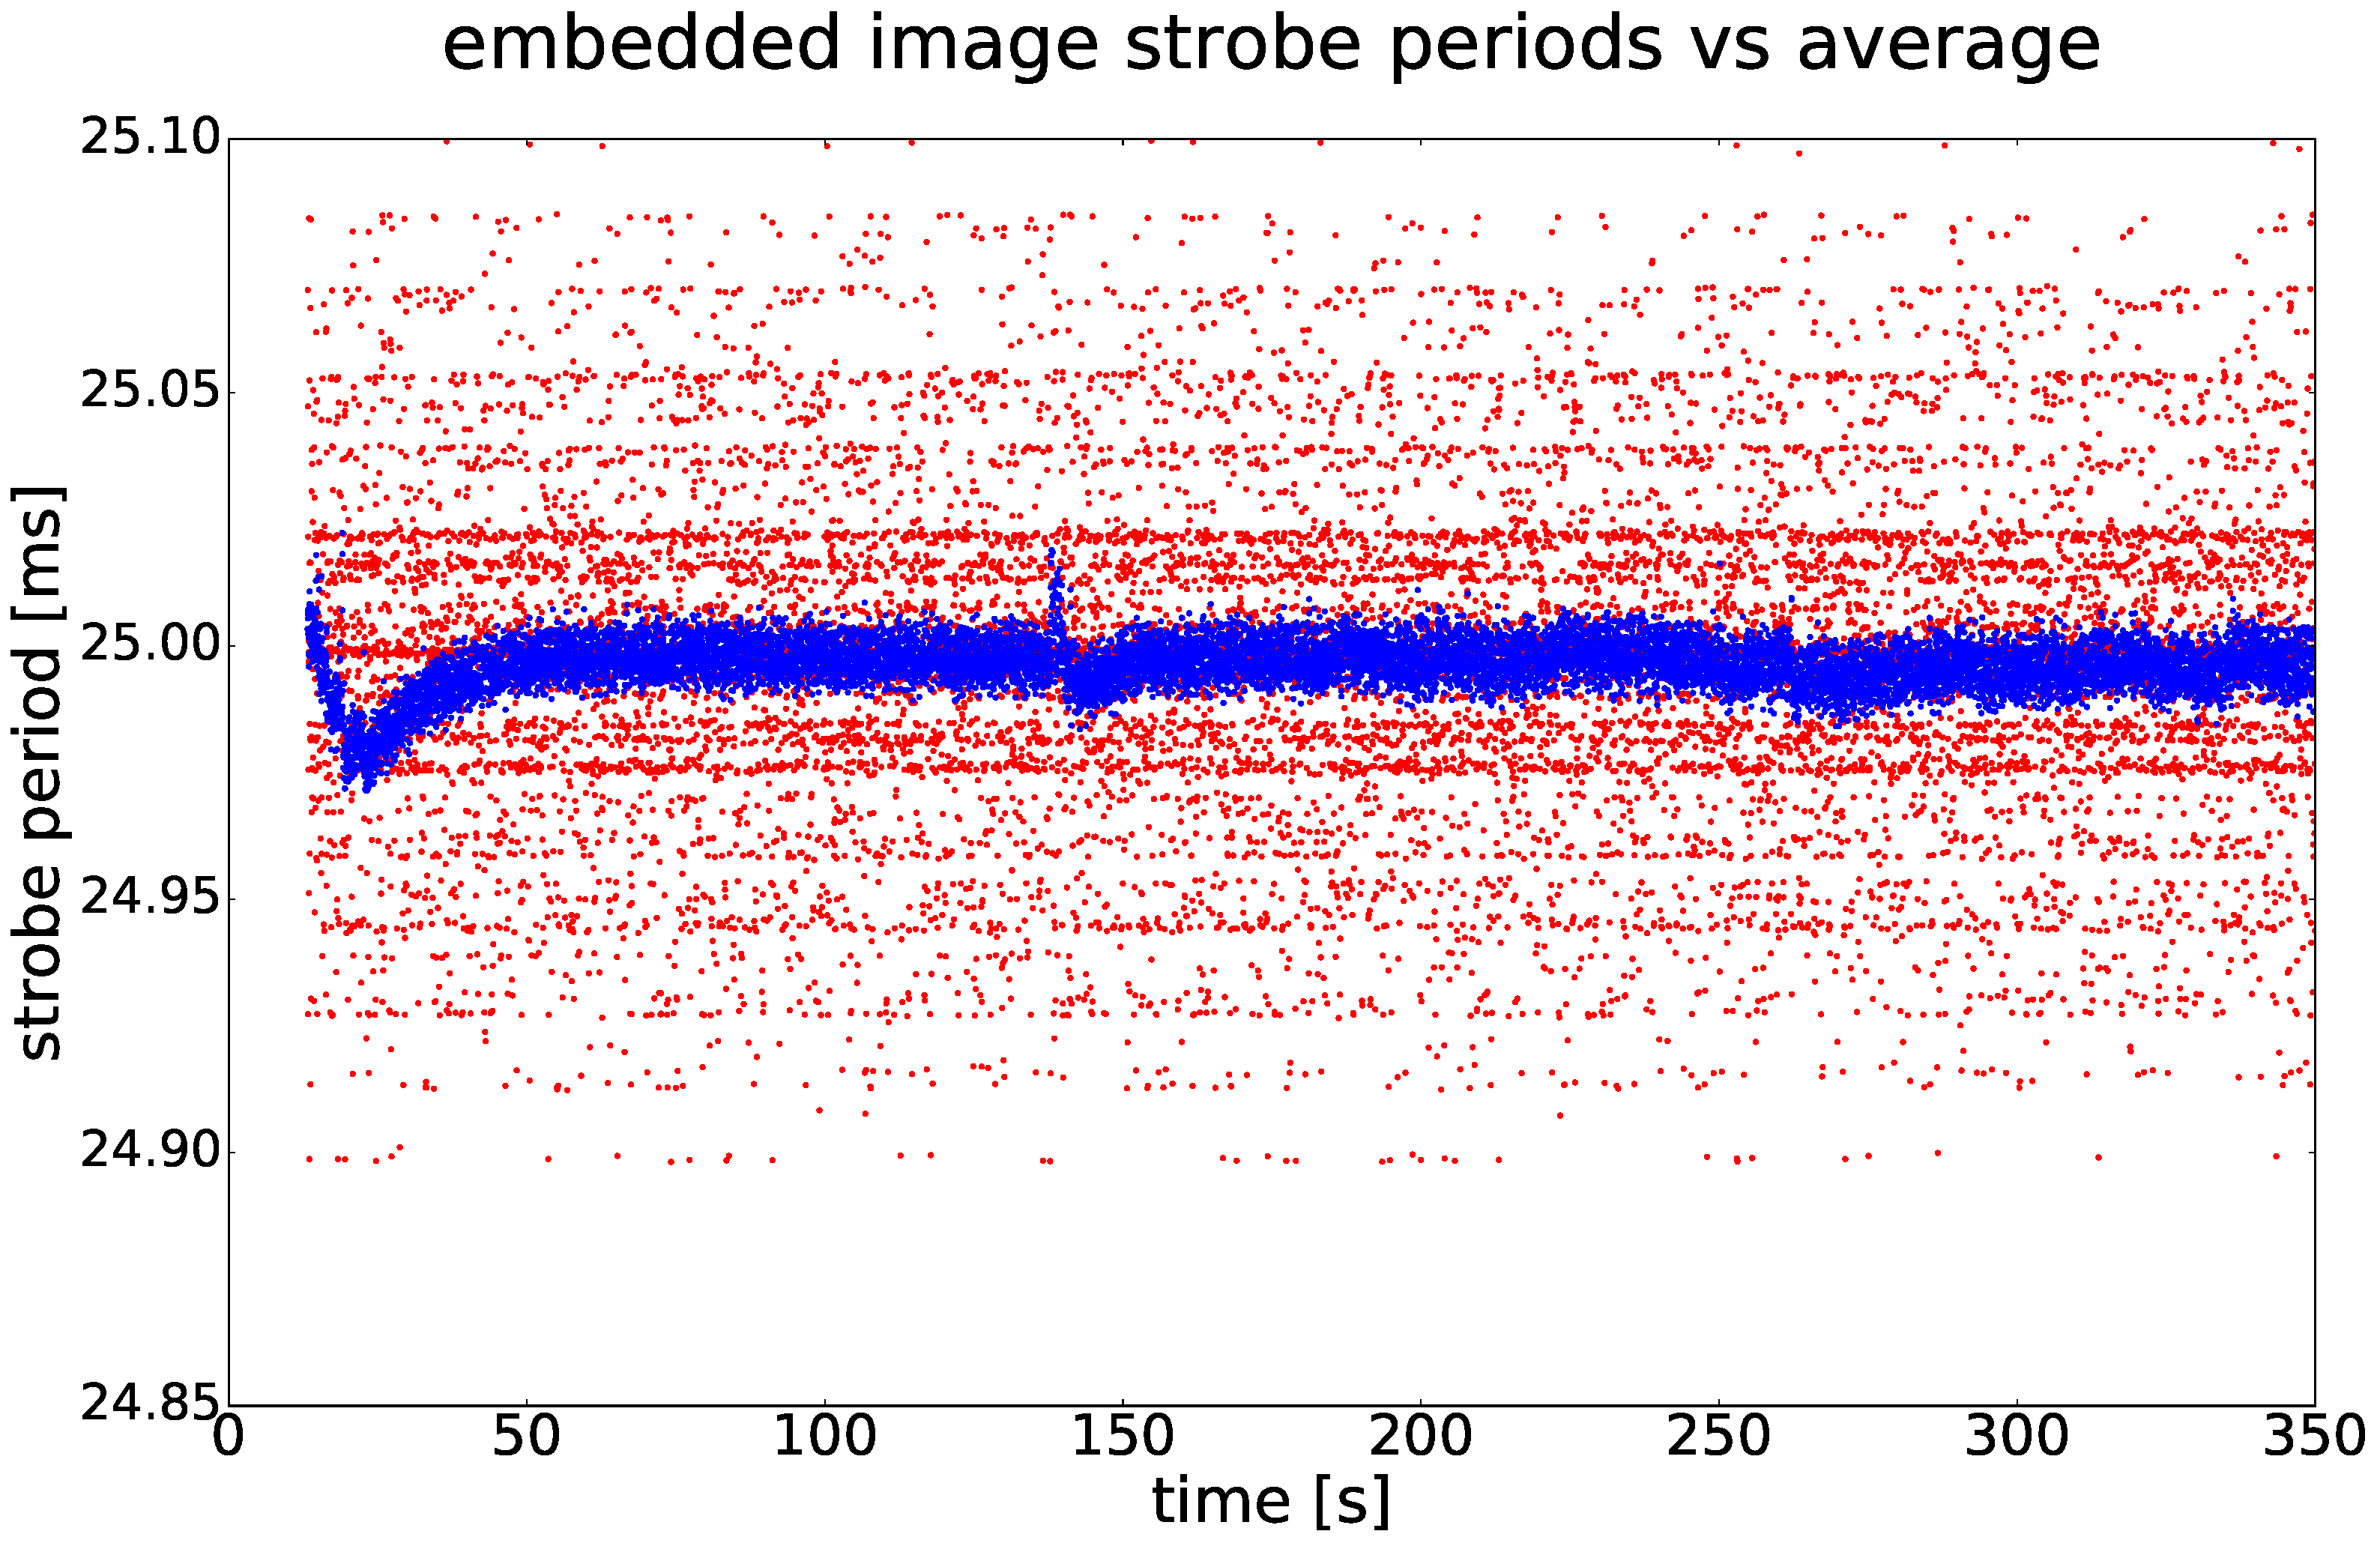
\includegraphics[width=\linewidth]{figures/embedded_vs_avg.pdf}
        \caption{Red dots: strobe periods $\eztime{n}-\eztime{n-1}$,
          computed from embedded image time stamps. Blue dots:
          $\dt$, calculated as moving average over all camera strobe periods.}
    \label{fig:embed_dt}
\end{figure}

After the start of the camera drivers, it takes about 30-50 seconds for
all cameras to produce frames at a reliable frame rate and for frame
drops to become less frequent. To decide when this warm up period has
ended, and  $\dt$ has stabilized, we compute another
moving average, but this time for the relative error from the currently
estimated mean:
\begin{equation}
V_n = V_{n-1} (1 - \alpha) + \alpha \left(\frac{\dtn{n} -
  \dtn{n-1}}{\dtn{n}}\right)^2\ .  
\end{equation}
$V$ measures something similar to the variance of the
updates to the average. When those updates are less than 1\%,
i.e. when $V_n < 0.01^2$, we consider the warm up period complete.


\subsection{Maintaining per-camera estimated pulse time}

Once a stable strobe period $\dt$ is available, one can use it to maintain an
estimate of the camera time for camera $i$:
\begin{equation}
\label{eq:camt}
\ttime{n} = \ttime{n-k} + k\dt + \beta(\atime{n} - (\ttime{n-k} + k\dt))\ ,
\end{equation}
where $k$ is the number of frames that have passed, as computed from Eq. \ref{eq:nframes}.
For the first frame, we set $\ttime{0} = \atime{0}$. The main innovation
to the camera time in Eq. \ref{eq:camt} obviously comes from $k\dt$, but
there is another term which mixes in a small amount ($\beta = 0.005$) of the difference
between the actual arrival time and the predicted camera time, thereby ensuring
that in the long run and on average, the camera time will not
drift away from the arrival time.
By means of Eq. \ref{eq:camt} we associate an arriving frame with the
time at which it was triggered at the camera, even if it arrives late due to temporary network
or CPU load. Due to the large reduction of jitter, the camera time $\ttime{}$ is
suitable for grouping frames by sync pulse, as shown in Fig. \ref{fig:arrival_vs_frame}.


\subsection{Assigning time stamps to frames}
When a frame arrives at the host and produces a new camera time
$\ttime{n}$ according to Eq. \ref{eq:camt}, it must then be associated with
a global time $T_n$ with which all frames belonging to this pulse $n$ are labeled.
For this purpose, a sorted list of times
$T_n$ is maintained, as well as an accumulator $\delta$.
At the start, $\delta$ is initialized to zero and the sorted list of
global times is cleared.

Upon arrival of a new frame, the sorted list is searched based on
$\ttime{n}$ and the following actions are taken:
\begin{itemize}
\item If the camera time of the arriving frame is close to a $T_n$ in
  the list, i.e.  $|T_n - \ttime{n}| \leq  \dt/2$, then
  it is associated with that $T_n$, and $T_n$ is the time stamp under
  which that camera frame will be published. Any difference is
  accumulated: $\delta \leftarrow \delta + (\ttime{n} - T_n)/N$, to be used
  subsequently.
\item If no list element close to $\ttime{n}$ is found, the camera frame
  establishes a new global time: $T_n
  =\ttime{n} + \delta$, which is entered into the sorted list, and $\delta$
  is reset to zero.
\end{itemize}
Without adding $\delta$, the time $T_n$ would be set to the time
$\ttime{n}$ of the first camera $i$ for which a frame arrives.
This would not be an issue if the arrival order of cameras were random.
In practice however we observe
persistent ordering in the arrival of frames. An obvious reason for
this are differences in shutter time, but thread scheduling policies,
interrupt priorities, FLIR driver implementation details, 
and the order in which incoming packets are processed by the network
interfaces could potentially all contribute to persistent
ordering. Adding $\delta$ causes $T_n$ to align with the mean of
the frame arrival times, and so improve the robustness of the
assignment.

\subsection{Monitoring correct association}
Given the large amount of noise in the arrival times of the frames, the
danger of persistently grouping the frames incorrectly, and thereby
generating systematically flawed data is very real. The method
presented in the preceeding subsections is not only robust to such failures, but can
easily produce statistics that directly demonstrate the validity of frame
associations. This can be done by simply computing for each camera $i$
the difference
\begin{equation}
^{(i)}\epsilon_n = (\atime{n} - T_n)/T_n
\end{equation}
between the arrival time of a frame, and the frame time $T_n$ that was
assigned to it. This quantity will obviously be very noisy, since the
frame time $T_n$ has low jitter, whereas $\atime{n}$ is
unfiltered. We therefore compute a moving average again:
\begin{equation}
\label{eq:eavg}
^{(i)}E_n = (1 - \gamma)\ ^{(i)}E_{n-1} + \gamma\ ^{(i)}\epsilon_n\ ,
\end{equation}
with a constant $\gamma = 0.025$ that corresponds to a time horizon of
about one second.

\begin{figure}[h]
	\centering
	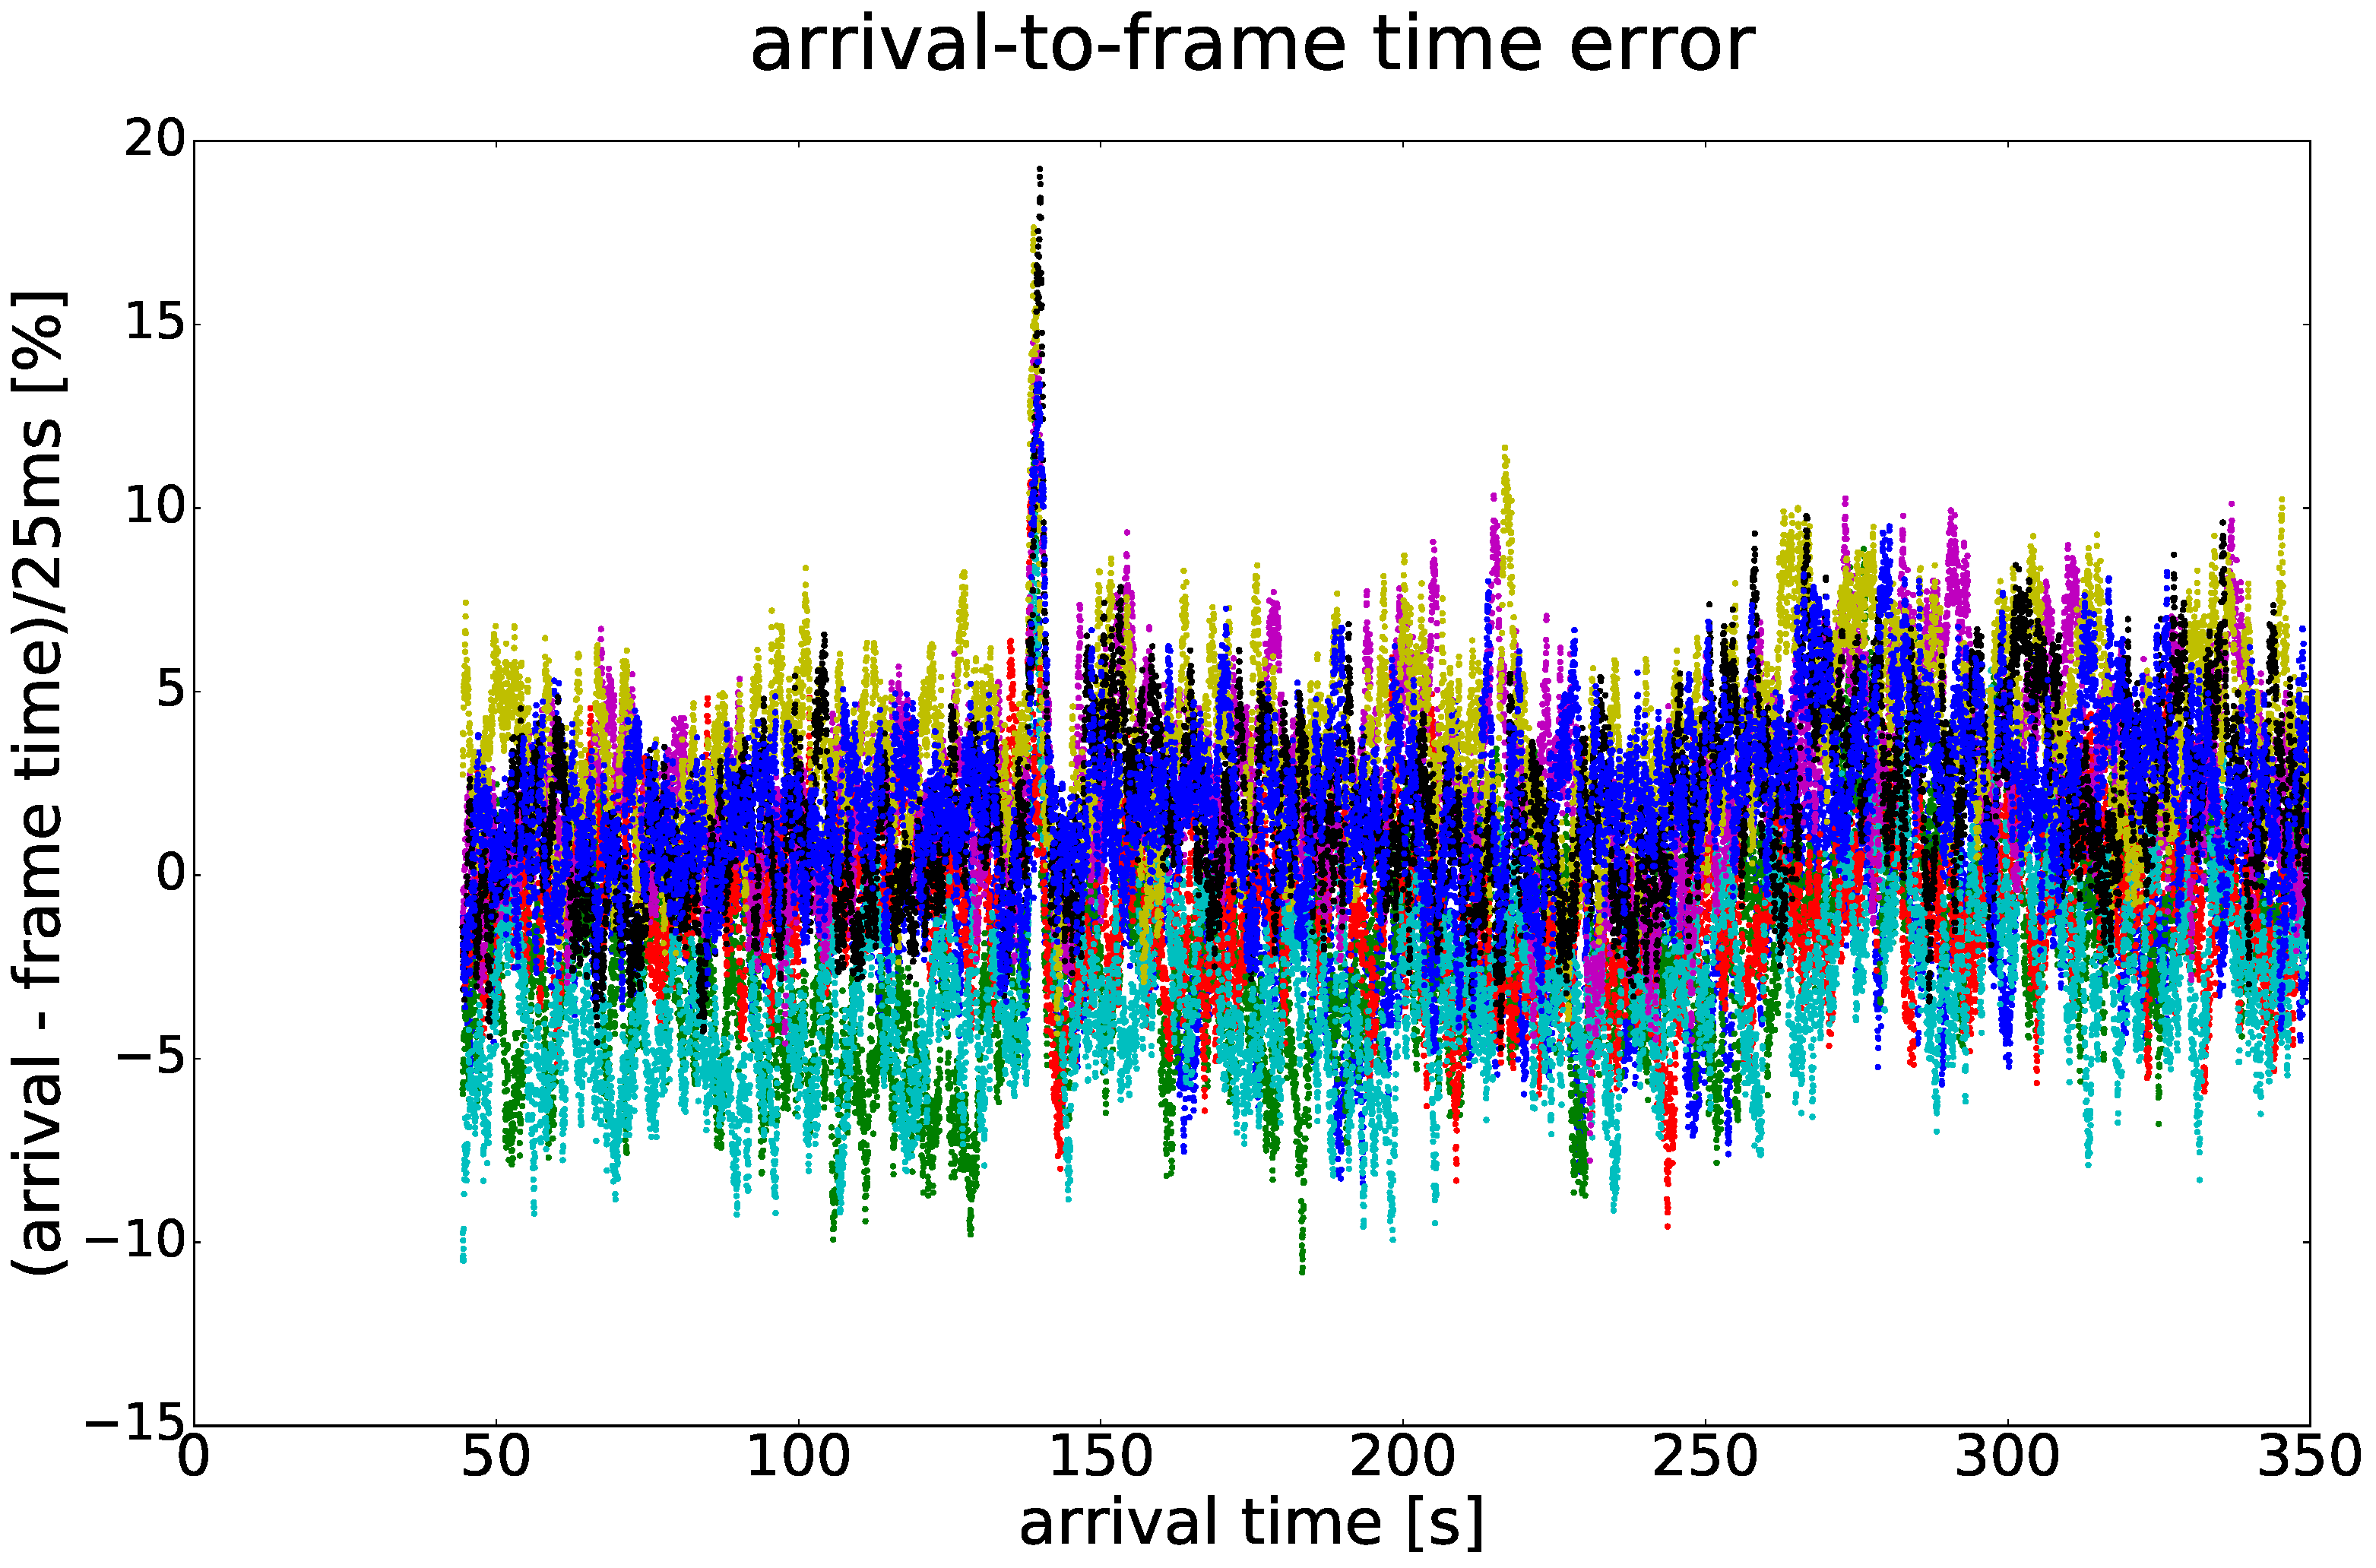
\includegraphics[width=\linewidth]{figures/monitoring.pdf}
        \caption{Plot of monitoring error $E$ (Eq. \ref{eq:eavg}) in
          \% of a full frame period, as a
          function of time for the post warm-up period. Each color
          corresponds to a different camera. Note how $E$ stays below
          20\% even when the load spike occurs at about 140s. One can also
          see that frames from certain cameras arrive consistently
          earlier than from others.}
    \label{fig:monitor}
\end{figure}

As Fig. \ref{fig:monitor} shows, the 1-second averaged error $E$ between
frame arrival time and frame time fluctuates between about -10\% and
+10\% of a full frame period (25ms). When a sudden load is put on the
system, $E$ can spike up to about 20\%, but quickly recovers.

In the actual implementation of CamSync, the averaged error $E$, along
with its standard deviation, are printed out once a minute. Failure to
pass other sanity checks (e.g. the same frame time being assigned to
consecutive frames for the same camera) are reported as well.

\section{Auto exposure}
\newcommand{\Bdes}{B_{\mathrm{des}}}
\newcommand{\Bcurr}{B_{\mathrm{curr}}}
\newcommand{\Bthresh}{B_{\mathrm{thresh}}}
\newcommand{\Scurr}{S_{\mathrm{curr}}}
\newcommand{\Smax}{S_{\mathrm{max}}}
\newcommand{\Gmax}{G_{\mathrm{max}}}
\newcommand{\Gcurr}{G_{\mathrm{curr}}}

\label{sec:auto_exposure}
The FLIR/PointGrey computer vision cameras used for our experiments
have a built-in auto exposure algorithm. However, auto exposure mode
is incompatible with hardware based shutter triggering, requiring
the implementation of an external software based exposure control.

For completeness, we describe the simple exposure control scheme
\cite{Liang2007} that 
is implemented in CamSync. The control algorithm adjusts both the
shutter time $S$ and the gain $G$. Gain is only used when the target
brightness cannot be reached by increasing the shutter time.

When a frame is received for camera $i$, the intensity values of the
pixels at every 32nd row and every 32nd  column of the image (in raw
Bayer format) are averaged. At 1920x1200 resolution, this equates to
2250 pixels that are sampled, and takes a negligible amount of CPU
time. The so computed image brightness $B$ is in the range of 0 to
255. If $B$ deviates by more than $\Bthresh$ (typically set to 10) from the
brightness target $\Bdes$ (typically about 90), then either shutter or
gain settings are updated.

Let $\Scurr$ denote the currently effective shutter time.
If $\Scurr$ is less than the configured maximum
shutter time $\Smax$ then the new commanded shutter speed is:
\begin{equation}
 S = \mathrm{min}(\Scurr \frac{\Bdes}{\Bcurr},\Smax)\ .
\end{equation}

If $\Scurr = \Smax$, gain control is used to reach the desired
brightness:
\begin{equation}
 G = \mathrm{min}(\Gcurr + 10 \log_{10}(\Bdes/\Bcurr),\Gmax)\ .
\end{equation}
Note that here the gain is expressed in decibels (db).

The commands to update gain or shutter speed are sent immediately
after the frame has been processed. However a few frames will elapse
until the driver's commands reach the camera. For
this reason the CamSync implementation will wait for a configurable
number of frames before it begins to evaluate the image brightness
again.

\section{Multithreading}
Since the synchronization method described in Sec. \ref{sec:sync_algo}
relies heavily on the arrival timestamps $\atime{}$ it is important
that incoming images are time stamped immediately before further
processing. This section describes how multithreading can be used to
accomplish this.

Fig. \ref{fig:multithreading} provides an overview of the
architecture. A separate polling thread is started for each camera,
and performs a blocking call to the FLIR/PointGrey FlyCapture driver API
to receive an image for the respective camera.
When the call returns, the polling thread immediately records the
arrival time stamp, updates the exposure settings if required, and
adds the image, together with the arrival time stamp, to the front of
a global synchronization queue. This is a very light weight operation
and requires only a short amount of time, thus ensuring that there is
very little resource contention, and none of the polling threads are
prevented from immediately entering the next blocking driver call.

A single synchronization thread operates on the synchronization
queue and computes the frame time stamps as described in
Sec. \ref{sec:sync_algo}. Finally, the time stamped frames are entered into a 
per-camera queue that compresses and publishes the image, thereby
making it available to subscribers on the ROS network.

\label{sec:multithreading}
\begin{figure}[ht]
	\centering
	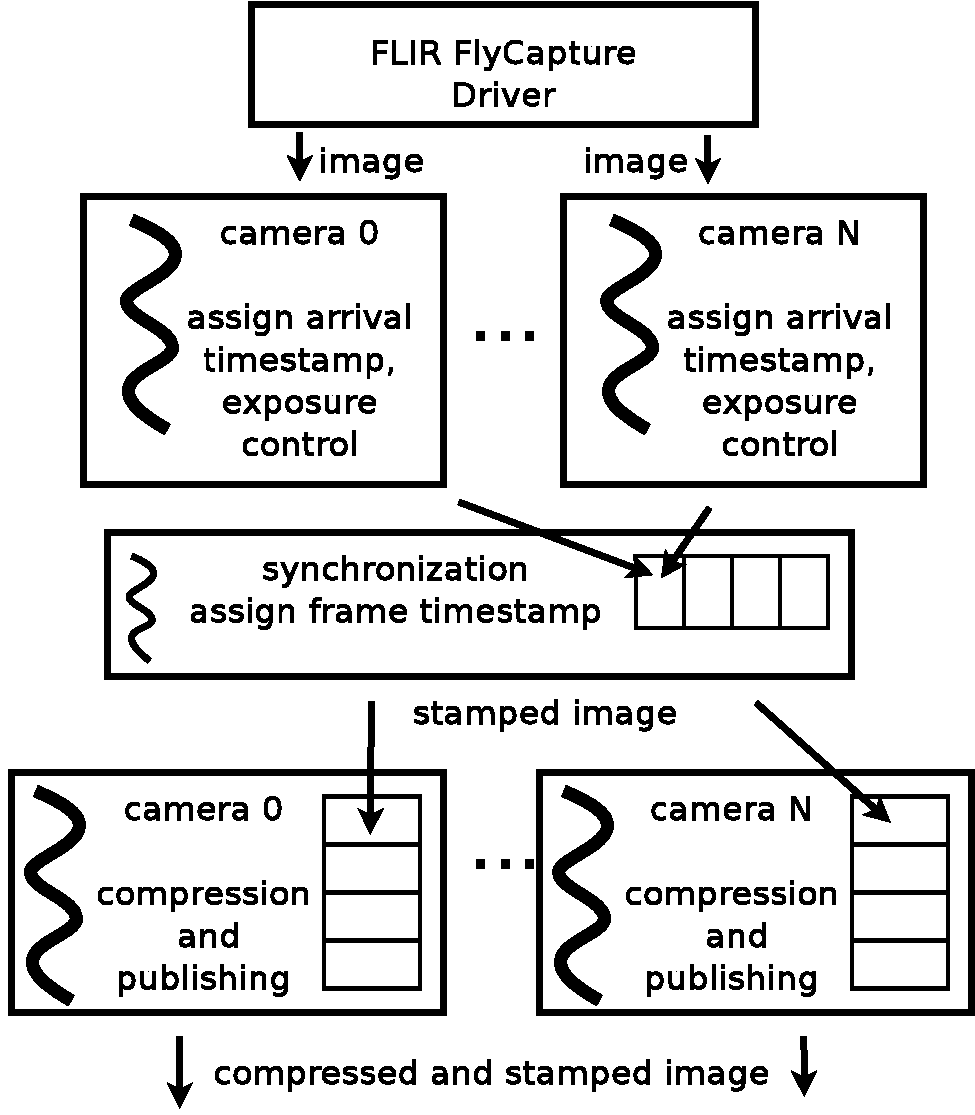
\includegraphics[width=\linewidth]{figures/threading.pdf}
        \caption{Multithreading: one thread per camera receives the
          image from the driver with a blocking call, puts on the
          arrival timestamp, updates exposure settings, and enqueues
          the image for the synchronization thread to process. Once
          the frame time stamp has been determined, the image is
          entered into a per-camera queue for compression and publishing.}
    \label{fig:multithreading}
\end{figure}

\section{Conclusion}
In this work, we show how synchronized camera images from a
multi-camera system can be reliably associated
with the synchronization pulses that triggered them. Our method
performs well under high jitter and does not require synchronized camera clocks. We
provide implementation details and demonstrate how this method works
for a multi-view system of 8 GigE cameras. The described algorithm is
implemented in CamSync, an open source ROS node available at 
\href{https://github.com/daniilidis-group/cam_sync}{https://github.com/daniilidis-group/cam\_sync}.


\bibliographystyle{IEEEtran}
\bibliography{camsync}

%\balance


\end{document}
